\chapter{Methodology} % Main chapter title
\label{Chapter4}

Having established context for the dataset chosen for our analysis, Chapter \ref{Chapter4} looks into the methodology adopted in this thesis. We begin this chapter by outlining the overall modelling approach (Section \ref{sec:4 Modelling Approach}) that provides a high-level view of our analysis, encompassing the general idea and process in formulating the individual recommendation model. After this overview, we look in detail at the NCF algorithm (\ref{sec:4 Neural Collaborative Filtering} - a recently implemented approach that leverages deep learning algorithms for collaborative filtering. This section will cover the background of NCF, the algorithm formulation, the neural network architecture, model training process as well as how we incorporated the review text and sentiments into the models. After this, in Section \ref{sec:Benchmark Models}, we clearly establish and describe the benchmark models used for comparison with the NCF models. The three benchmark models are discussed, and their underlying algorithms briefly explained. Additionally, Section \ref{sec:Evaluation} addresses the evaluation criteria that will be used to assess the performance of our recommender models. The chapter concludes with Section \ref{sec:Conclusion for Methodology} giving a summary of details discussed in this chapter.

\section{Modelling Approach}
\label{sec:4 Modelling Approach}

One can view the recommendation problem as a prediction problem. Within this framework, a pool of users interact with a diverse range of items, presenting the challenge of predicting a user's rating for an unseen item. The predictive algorithm is simply some tool that uses the users’ historical purchases (or reviews in our case) to learn the users’ preferences to be able to predict \textit{liking} for future items. To augment the predictive algorithm, we propose supplementing the algorithm with additional information, namely review text and sentiment. The conjecture is that this augmentation could yield more accurate predictions and provide users with recommendations that resonate with their preferences more closely. To effectively explore this hypothesis, we devise a comprehensive approach that balances the workings of collaborative filtering, neural network architectures, and the incorporation of additional information. The details of which shall be described in this section.

\subsection{Formulating the Problem}
\label{subsec:4 Formulating the Problem}

For recommender systems, the problem space can be formulated as a matrix of users versus items, with each cell representing a user’s rating on a specific item \cite{jannach2010recommender}. That is, the users are represented as rows while the products are represented as columns, each cell value points to the ratings given to the product by a particular user. Under this formulation, the problem is to predict the values for specific empty cells (i.e. predict a user’s rating for an item they have not rated). We acknowledge the sparsity of this matrix, a characteristic often present in e-commerce data, as discussed in Section \ref{subsec: Sparsity}. Given the vast array of items available, each user interacts with only a fraction of the total amount of products. A depiction of a user-item matrix is shown in Table \ref{tab:user_item_matrix}. The blank spaces indicates the user has not reviewed (or purchased) the item before.

\begin{table}[h]
    \centering
    \begin{tabular}{|c|c|c|c|c|c|c|}
    \hline
     & Item 1 & Item 2 & Item 3 & Item 4 & $\cdots$ & Item $K$ \\
    \hline
    User 1 & 3 & 2 &  &  & $\cdots$ &  \\
    User 2 & 4 &  &  & 4 & $\cdots$ & 5 \\
    User 3 & 5 & 5 & &  & $\cdots$ & 5 \\
    User 4 & 5 & & 2 &  & $\cdots$ &  \\
    User 5 &  & 5 & &  & $\cdots$ & 3 \\
    User 6 & 5 & 4 & &  5& $\cdots$ & \\
    $\vdots$ & $\vdots$ &  $\vdots$ & $\vdots$ &  & $\cdots$ & $\vdots$ \\
    User $N$ & 4 & & 5 &  & $\cdots$ & 4 \\
    \hline
    \end{tabular}
    \caption{User-Item Matrix}
    \label{tab:user_item_matrix}
\end{table}

Formally, we denote the user-item interaction matrix as $\mathbf{R}$, where $r_{ij}$ represents the rating user $i$ gives to item $j$. Furthermore, we introduce the predicted interaction matrix, denoted as $\mathbf{\hat{R}}$, which will contain our model's estimations of the user-item interactions. Other notations will be introduced throughout this chapter where required. Our recommender system paradigm falls within collaborative filtering, which (as mentioned in Section \ref{sec:2 Collaborative Filtering}) leverages the collective wisdom embedded in user-item interactions to discern inherent patterns or preferences, enabling the system to make predictions for unobserved user-item pairs \cite{koren2009collaborative}. Effectively, a collaborative filtering system will navigate $\mathbf{R}$, the user-item matrix, aiming to uncover latent relationships and preferences by assessing how users with similar tastes have rated similar items. The intuition is that users who have historically exhibited analogous preferences are likely to align in their ratings for items they have not yet interacted with \cite{koren2009collaborative}. The goal is to completely populate the empty user-item pairs in $\mathbf{R}$ to generate $\mathbf{\hat{R}}$.

Fundamentally, this is the problem we aim to solve. We seek to build several models (using different algorithms) that can accurately predict the ratings for unseen user-item pairs and then compare their performance. The manner in which these models learn to estimate these ratings follows the collaborative filtering approach. One such model is a NCF recommender system, which use neural networks to directly learn representations of users and items from the user-item interaction matrix $\mathbf{R}$, and then uses these representations to predict the ratings for unseen user-item pairs \cite{he2017neural}. The next subsection looks at how we solve the prediction problem specifically using this model.

\subsection{Implementation and Approach}
\label{subsec:4 Implementation and Approach}

Initially, our focus is on constructing a neural collaborative filtering (NCF) model using only the available ratings. Subsequently, we progress to integrating review text and sentiments into our model sequentially. In this initial phase (using ratings only) we initiate our modelling process by transforming the cleaned data into a user-item ratings matrix. Mathematically, this translates to defining $U$ as the set of users, $I$ as the set of items, and $\mathbf{R}$ as the user-item ratings matrix $\mathbf{R} \in \mathbb{R}^ {\lvert U \rvert \times \lvert I \rvert}$. The subsequent steps in constructing the various recommender models in this thesis, including the neural collaborative filtering and benchmark models, follow identical procedures:

\begin{enumerate}
    \item partition the user-item matrix
    \item train an algorithm using training set
    \item optimise an algorithm using validation sets (if required)
    \item evaluate an algorithm using testing set
\end{enumerate}

Thus, having converted the cleaned data into a user-item ratings matrix, we proceed to partition the matrix following the methods detailed in Section \ref{sec:3 Data Partitioning}. The partitioning strategy involves randomly selecting $5$ ratings from each user and assigning them to either the validation or testing set. Specifically, the validation set comprises of 7 336 ratings, and the testing set consists of 11 004 ratings. This ensures that our models are trained on a minimum of 7 ratings per user (training data is approximately 64 799 reviews).

With the data appropriately partitioned, we are now poised to integrate the recommender algorithm for training. The construction of the recommenders were all done from fundamentals, using Python and the TensorFlow\footnote{TensorFlow is an open-source machine learning framework developed by Google. It is widely used for building and training machine learning models.} library. Each recommender was trained using the training data. We used the validation data to optimise the hyperparameters of the NCF model only. The decision to not optimise the parameters for the benchmark models shall be discussed in Section \ref{subsubsec:4 Hyperparameter Tuning}. The testing data was used to evaluate the performance of the models.  The models are assessed based on their predictive accuracy (how accurately they can predict unrated items) and their ability to recommend top-$n$ items (how relevant the recommendations are) to users. The specific evaluation metrics used to assess the performance of the models are discussed in Section \ref{sec:4 Evaluation}.

This process of training, optimising (for NCF), and evaluating is iteratively repeated for scenarios (the NCF models) where we incorporate review text and, subsequently, review sentiment. It is imperative to conduct these steps separately and then in combination to discern the impact of additional information (features) on the model's performance. This approach allows us to assess whether the inclusion of review text and sentiment enhances the predictive capabilities of our recommender system. As such, we will have three different NCF models - more on this in the next section. 

The workings and approach described in this section is summarised by the flow chart in Figure \ref{fig:flowchart of process}. As we embark on the development of the NCF model, the next section will provide some background into neural networks, providing a high-level overview of how they work. Subsequently we will look at NCF, exploring its architecture, training process, and how it operates within the general collaborative filtering approach.

\begin{figure}[h]
    \centering
    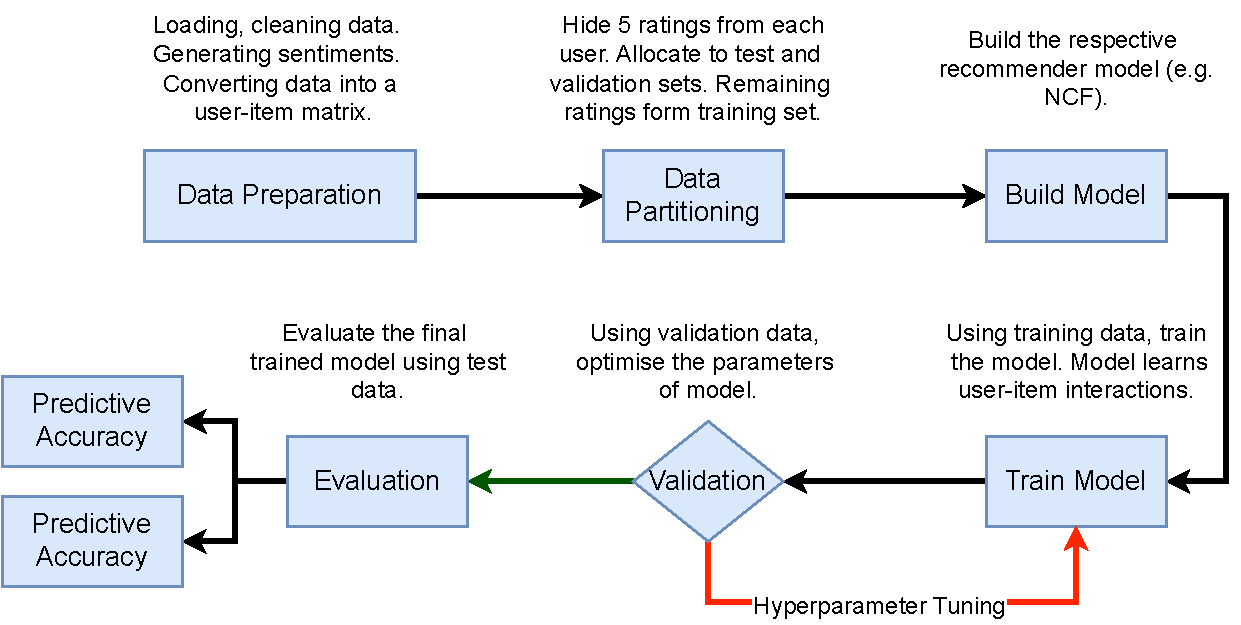
\includegraphics[width=0.9\textwidth]{Figures/flowchart of model process-4.pdf} % Adjust the width as needed
    \caption{Flowchart outlining the general process followed in applying and evaluating the recommender models.}
    \label{fig:flowchart of process}
  \end{figure}
  
  \section{Neural Networks}
  \label{sec:4 Neural Networks}

Neural networks have become a cornerstone of modern artificial intelligence and machine learning \cite{abdi1999neural}. They have evolved from over the past two decades to complex deep learning architectures that are capable of learning complex patterns and making predictions from data \cite{gurney2018introduction}. At its core, a neural network consists of interconnected nodes, or neurons, organized into layers \cite{abdi1999neural}. Figure \ref{fig:neural_network} provides a visual representation of a neural network, showing an example of an input layer, hidden layers, and an output layer.

\begin{figure}[h]
    \centering
    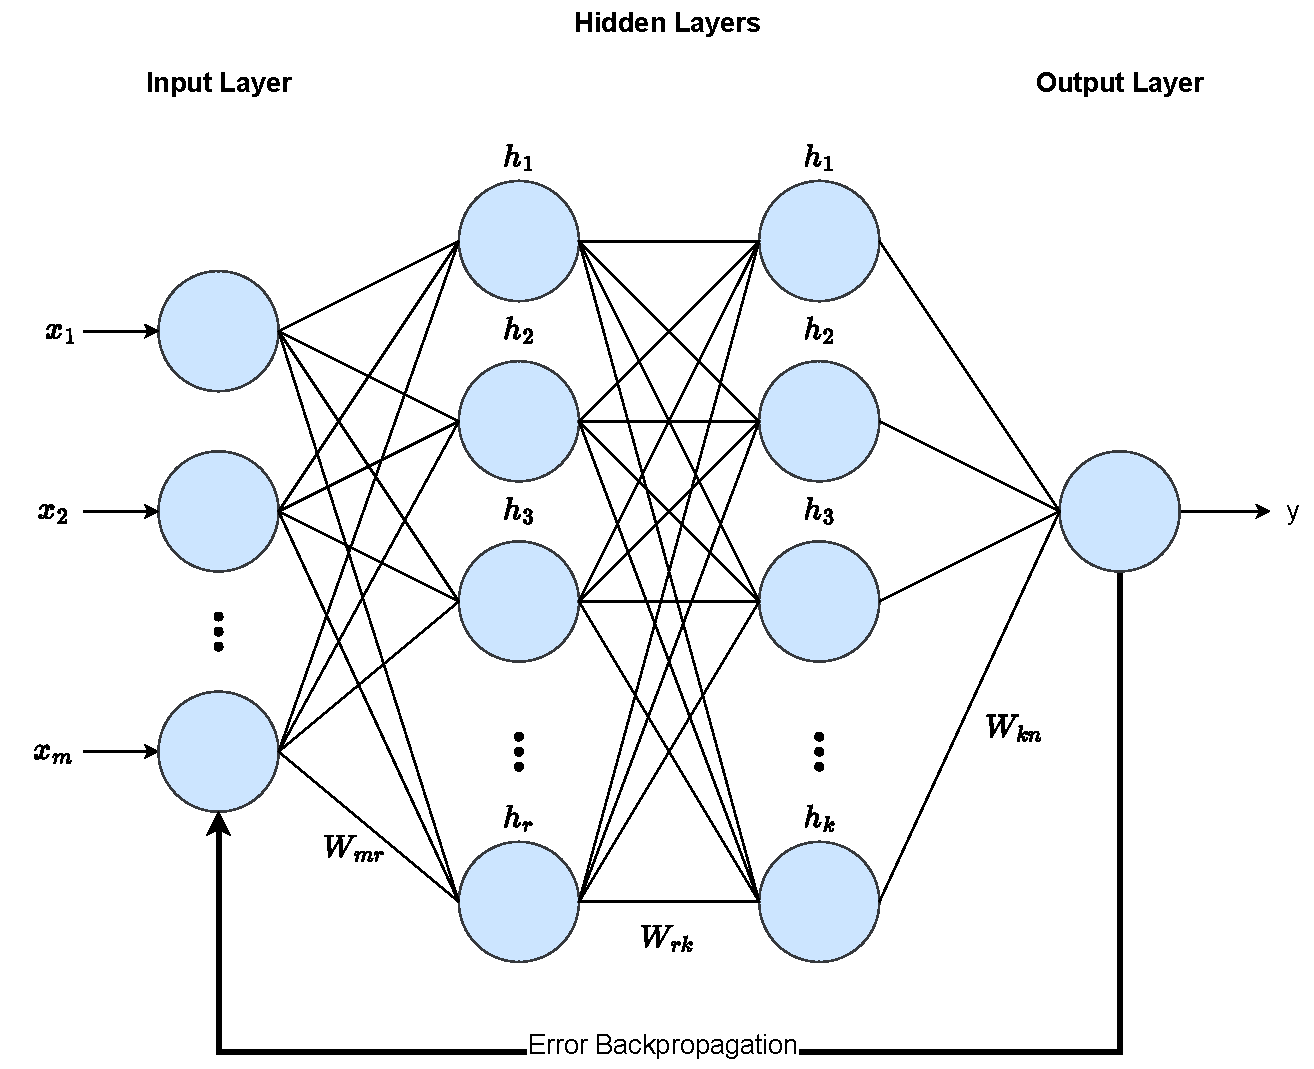
\includegraphics[width=0.9\textwidth]{Figures/flowchart of model process-Neural Nets.pdf} % Adjust the width as needed
    \caption{Neural Network Architecture showing an example of an input layer, hidden layers, and an output layer.}
    \label{fig:neural_network}
  \end{figure}

Neural networks, as mentioned, are composed of interconnected nodes (called neurons) that work together to process complex data inputs and produce an output \cite{gurney2018introduction}. The nodes are organised into layers, with each layer performing a specific function. The input layer receives the data ($x$), the hidden layers process the data, and the output layer produces the result ($y$). The connections between the nodes are weighted ($W$), and these weights are adjusted during the training process to improve the accuracy of the model \cite{abdi1999neural}. 

Specifically, the training process involves feeding the network with data and adjusting the weights to minimise a loss function, which generally measures the difference between the predicted output and the actual output \cite{abdi1999neural}. This is done using an optimisation algorithm to find the optimal weights that minimise the error. The weights are adjusted iteratively until the model produces the desired or optimal output. The process of adjusting the weights is known as backpropagation, and it is a fundamental concept in training neural networks. The backpropagation algorithm calculates the gradient of the loss function with respect to the weights and uses this information to update the weights. This process is repeated until the model converges to an optimal set of weights that minimises the error (i.e., the model learns the patterns in the data). Effectively, backpropagation entails propagating the error backwards through the network to adjust the weights and improve the model's performance \cite{abdi1999neural}. 

In neural networks, the weights are the parameters that the model learns during training \cite{gurney2018introduction}. Neural networks also have many hyperparameters that need to be set before training, such as the number of layers, the number of neurons in each layer, the activation functions, and the learning rate. These hyperparameters can significantly affect the performance of the model and need to be tuned carefully to achieve the best results \cite{gurney2018introduction}. Table \ref{tab:hyperparameters} provides a summary and description of common hyperparameters that need to be set when training a neural network. To select the optimal combination of hyperparameters, a grid search can be performed \cite{gurney2018introduction}. A grid search involves training the model with different combinations of hyperparameters and selecting the one that produces the best results (i.e., the lowest error) \cite{gurney2018introduction}.

\begin{table}
    \centering
    \begin{tabular}{|c|c|c|}
    \hline
    Hyperparameter & Description & Example Values \\
    \hline
    Learning Rate & Step size for updating weights & 0.001, 0.01, 0.1 \\
    Number of Layers & Number of layers in the network & 1, 2, 3 \\
    Number of Neurons & Number of neurons in each layer & 32, 64, 128 \\
    Activation Function & Function applied to the output of a neuron & ReLU, Sigmoid, Tanh \\
    Batch Size & Number of samples processed at once & 32, 64, 128 \\
    Optimizer & Algorithm used to update weights & Adam, SGD, RMSprop \\
    Loss Function & Function used to measure the error & MSE, MAE, Cross-Entropy \\
    Epochs & Number of times the model sees the data & 10, 50, 100 \\
    \hline
    \end{tabular}
    \caption{Hyperparameters for training a neural network}
    \label{tab:hyperparameters}
\end{table}

Each hyperparameter plays a crucial role in the performance of the model. The learning rate determines how quickly the model learns the patterns in the data. A high learning rate can cause the model to converge too quickly and miss important patterns, while a low learning rate can cause the model to converge too slowly and take longer to learn the patterns. The number of layers and neurons in each layer also affect the model's performance. A deeper network with more layers can learn more complex patterns, but it can also be more prone to overfitting \cite{zhang2018improved}. The activation function is another important hyperparameter that determines how the output of a neuron is transformed. Common activation functions include ReLU, Sigmoid, and Tanh. The batch size is the number of samples processed at once during training. A larger batch size can speed up training but can also require more memory \cite{diaz2017effective}. The optimiser is the algorithm used to update the weights during training \cite{zhang2018improved}. Common optimizers include Adam, SGD, and RMSprop. The loss function is used to measure the error between the predicted output and the actual output. Common loss functions include Mean Squared Error (MSE), Mean Absolute Error (MAE), and Cross-Entropy. The number of epochs is the number of times the model sees the data during training \cite{diaz2017effective}. Specifically, one epoch is one pass through the entire dataset. Training for more epochs can improve the model's performance, but it can also lead to overfitting \cite{gurney2018introduction}. 

Neural networks have been widely used in various fields, including computer vision, natural language processing, and recommendation systems. They have been shown to be effective in learning complex patterns and relationships in data, making them suitable for tasks that involve high-dimensional data and non-linear relationships. In the context of recommendation systems, neural networks have been used to learn user and item representations from user-item interactions and make predictions about user preferences - as mentioned in Section \ref{sec:2 Deep Learning in Recommender Systems}. The next section will focus on the specifics of the neural collaborative filtering algorithm, which is a recommendation model that leverages neural networks to learn user and item representations and make predictions about user preferences.


\section{Neural Collaborative Filtering}
\label{sec:4 Neural Collaborative Filtering}

In this section, we focus on the details of NCF, providing first some high-level workings of the algorithm (Section \ref{subsec:4 Background}), then a comprehensive overview encompassing the algorithm's formulation (Section \ref{subsec:4 Algorithm Formulation for NCF}), the details of the training procedure (Section \ref{subsec:4 Model Training}) and model optimisation (Section \ref{subsec:4 Hyperparameter Tuning}). Following this, we discus the method in which the review text and sentiments are incorporated into the NCF model in Section \ref{subsec:4 Incorporating Text and Sentiments}, training and tuning results (Section \ref{subsec:4 Training Results}) and finally the specifications and architecture of the final models (Section \ref{subsec:4 Final Model Specifications}).

\subsection{Background}
\label{subsec:4 Background}

The advent of deep learning has marked a paradigm shift in various domains, demonstrating its prowess in extracting intricate patterns and representations from complex data \cite{steck2021deep}. While deep learning had been explored in recommender systems before, the paper by \cite{he2017neural} in 2017 holds significance as it delineates a generalised approach for integrating deep learning into recommender systems, specifically introducing Neural Collaborative Filtering (NCF). Serving as a guiding reference for this thesis, the work provides insights that aid in constructing, optimising, and making specification choices for our very own NCF model.

Traditional collaborative filtering methods, while effective, often struggle with capturing intricate user-item relationships \cite{steck2021deep}. Deep learning has the ability to model intricate relationships in high-dimensional spaces, presenting a compelling solution to this problem \cite{he2017neural}. NCF, as a deep learning-based recommender system, leverages neural networks to directly learn user and item representations from the user-item interaction matrix, enabling it to make predictions for unseen user-item pairs \cite{he2017neural}. The neural network architecture within NCF is designed to capture complex interactions, offering a flexible and possibly more accurate recommendation mechanism compared to traditional collaborative-based counterparts \cite{he2017neural}.

\subsection{Algorithm Formulation}
\label{subsec:4 Algorithm Formulation for NCF}

 An initial high-level overview of the algorithm is portrayed by Figure \ref{fig:NCF algorithm}, which we will make reference to often in this subsection as we build up and discuss the workings of the NCF algorithm.

\begin{figure}[h]
  \centering
  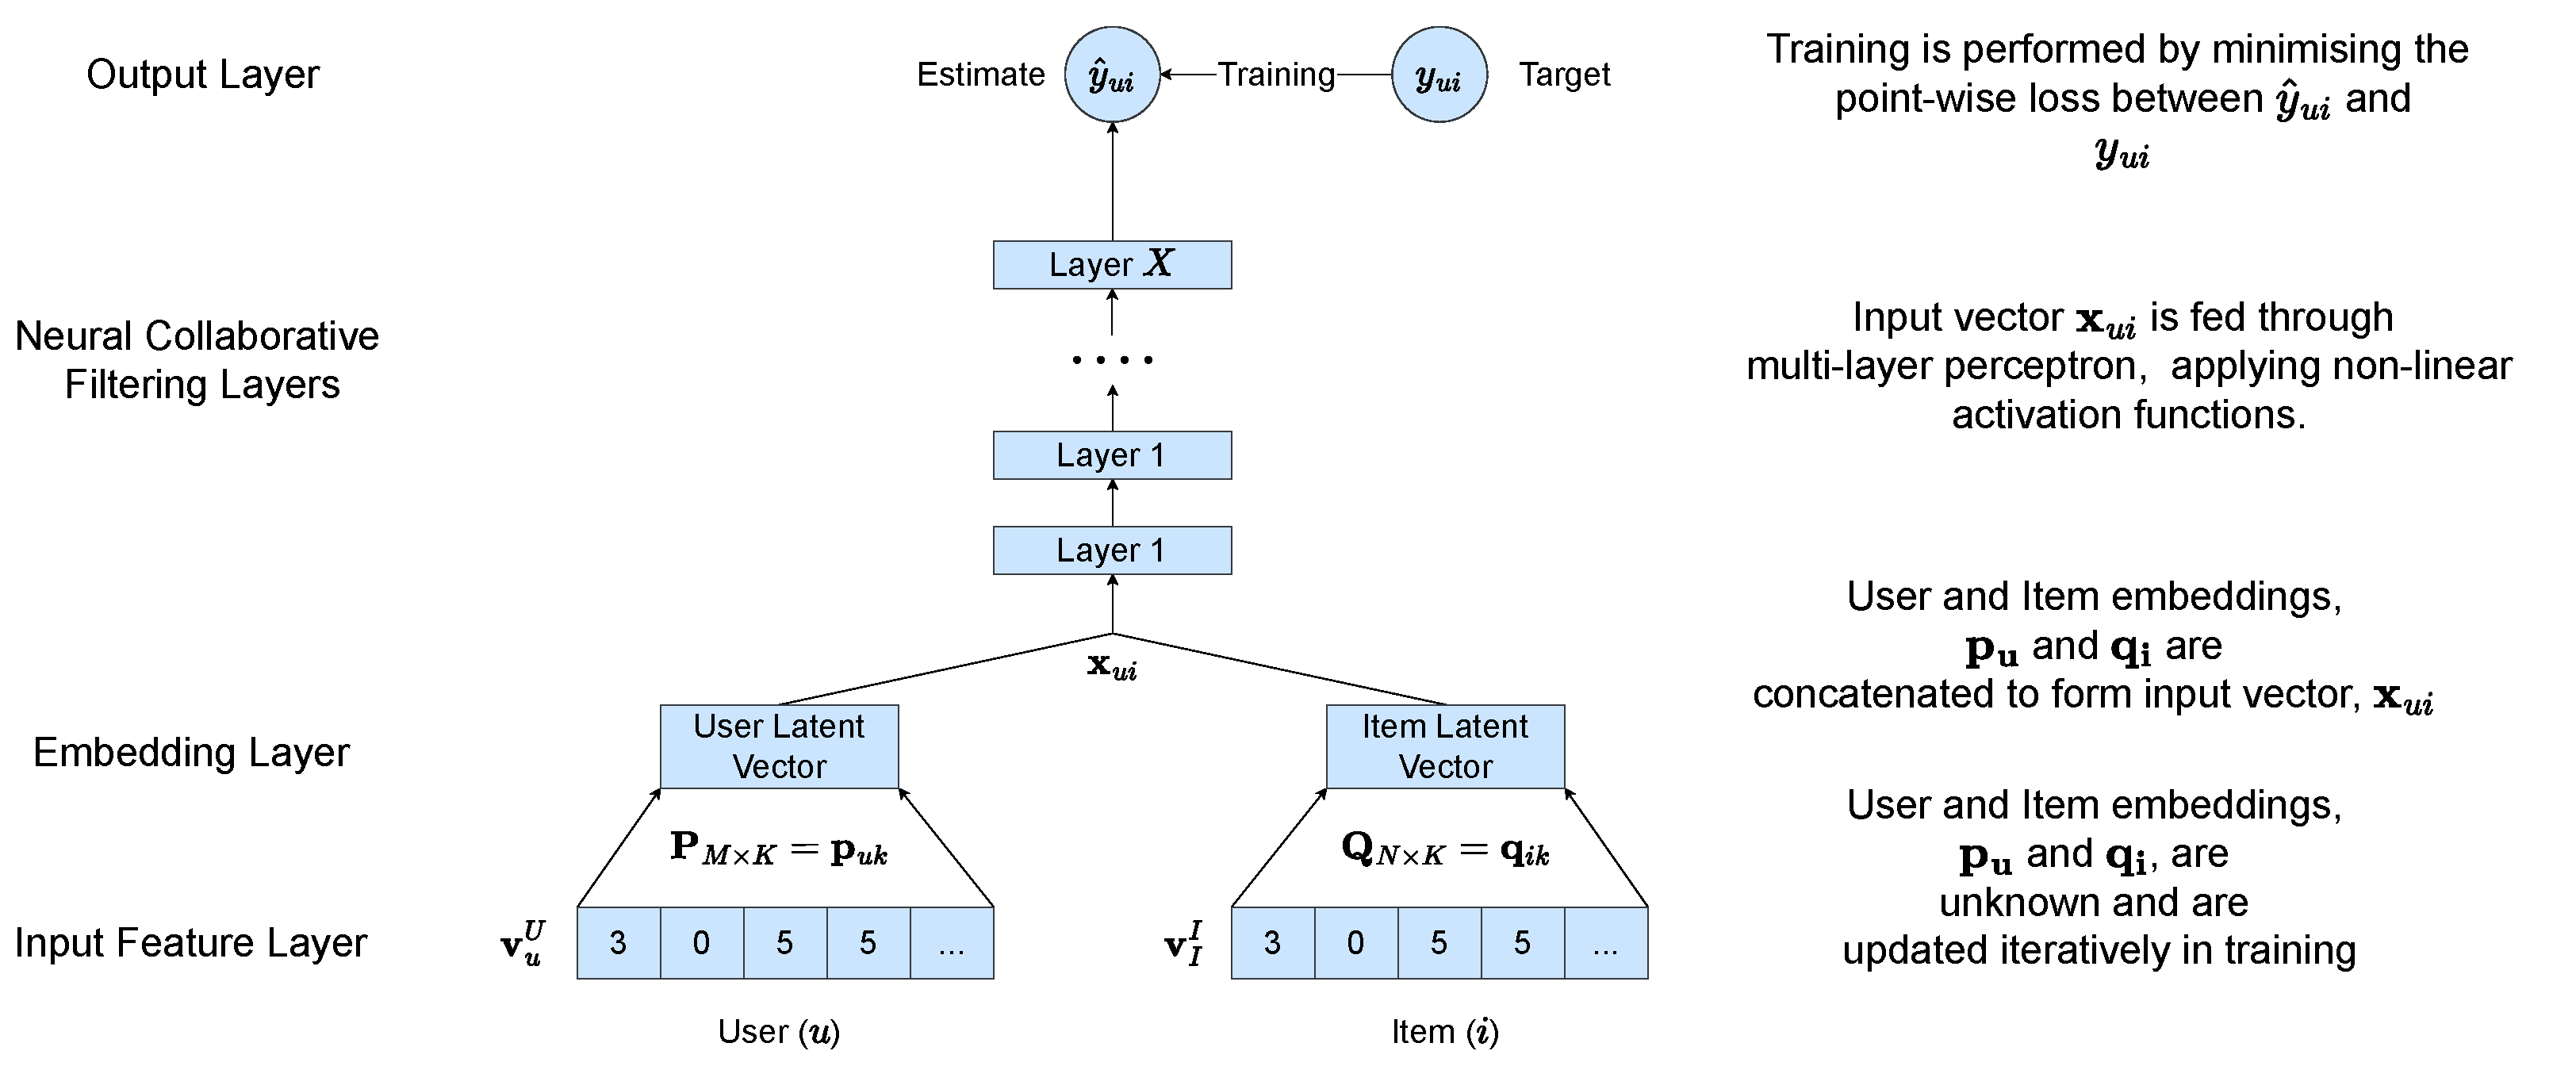
\includegraphics[width=0.9999\textwidth]{Figures/flowchart of model process-NCF-5.pdf} % Adjust the width as needed
  \caption{Neural Collaborative Filtering Algorithm.}
  \label{fig:NCF algorithm}
\end{figure}

Consider Figure \ref{fig:NCF algorithm}, the bottom input layer consists of two feature vectors $\mathbf{v}_u^U$ and $\mathbf{v}_i^I$ that describe user $u$ and item $i$ features, respectively. NCF initiates the recommendation process by embedding\footnote{Embedding is a technique used to represent categorical variables, such as users and items, as dense vectors in a continuous vector space. These embeddings capture the latent features and relationships between users and items, enabling the neural network to learn from their interactions.} users and item feature vectors ($\mathbf{v}_u^U$ and $\mathbf{v}_i^I$) into low-dimensional embeddings. For a user $u$ and an item $i$, the user and item embeddings are denoted as $p_u \in \mathbb{R}^d$ and $q_i \in \mathbb{R}^d$, respectively. These embeddings are initialised randomly and updated during the training process \cite{he2017neural}. The concatenation of user and item embeddings forms the input vector $x_{u i} \in$ $\mathbb{R}^{2 d} $ for the subsequent neural collaborative filtering layers. This is shown in the embedding layer, where the user and item embeddings ($p_u$ and $q_i$) are concatenated to form the input vector $\mathbf{x}_{ui}$ (for the neural network).

$$
x_{u i}=\text { Concatenate }\left(p_u, q_i\right) \forall u i
$$

 The input vector ($\mathbf{x}_{ui}$) is then fed into the neural collaborative filtering layers, which consist of multiple fully connected layers that learn the latent representations of users and items \cite{he2017neural}. Specifically, to permit a full neural network treatment of collaborative filtering, the NCF layers consist of multiple fully connected perceptrons\footnote{A perceptron is a single-layer neural network that can learn linear decision boundaries.} with non-linear activation functions such as rectified linear units (ReLU)\footnote{ The ReLU activation function is defined as $f(x) = \max(0, x)$.}. The activation functions are applied to the output of each perceptron, enabling the model to learn complex patterns and relationships in the data \cite{he2017neural}. Thus, we can view the multi-layer perceptron as a series of stacked layers, each applying non-linear transformations through activation functions, enabling the model to learn hierarchical feature representations  \cite{steck2021deep}. Effectively, through this architecture, the neural network learns the latent representations of users and items by transforming the input vector ($\mathbf{x}_{ui}$) through the multiple layers of non-linear transformations (output of one layer serves as the input of the next one) \cite{he2017neural}. The final output layer is the predicted score $\hat{y}_{u i}$ (i.e., the predicted rating of user $u$ for item $i$), and model training is performed by minimising the pointwise\footnote{Pointwise loss functions calculate the loss for each individual prediction separately.} loss between $\hat{y}_{u i}$ and its target value $y_{u i}$ \cite{he2017neural}.
 

 Formally, we can express the output of the neural network, denoted by $f\left(x_{u i}\right)$, as a series of ReLU activation functions applied to weighted sums. Let $f\left(x_{u i}\right)$ represent the output of the neural network, and $\hat{y}_ {u i}$ denote the predicted rating for user $u$ on item $i$.

\begin{equation}
    \label{eq:NCF layers output}
    f\left(x_{ui}\right) = \operatorname{ReLU}\left(W_l \cdot \operatorname{ReLU}\left(W_{l-1} \cdot \ldots \operatorname{ReLU}\left(W_1 \cdot x_{ui} + b_1\right) + b_{l-1}\right) + b_l\right).
\end{equation}
    
\begin{equation}
    \label{eq:output layer prediction}
    \hat{y}_{ui} = \left(f\left(x_{ui}\right)\right).
\end{equation}


Here, $W_l$ represents the weight matrix of the $l$-th layer, $b_l$ represents the bias vector of the $l$-th layer, and $\cdot$ denotes matrix multiplication. Equation \ref{eq:NCF layers output} denotes that the input $x_{ui}$ is passed through each layer of the neural network, with ReLU activation functions applied to the weighted sums at each layer. Equation \ref{eq:output layer prediction} shows that the final output $f\left(x_{ui}\right)$ represents the predicted rating $\hat{y}_{ui}$ for user $u$ on item $i$ - i.e., we apply a linear activation function\footnote{The linear activation function simply outputs the weighted sum of the inputs without applying any non-linear transformation.} to the output of the last layer to predict the rating.


Thus, we can formulate and generalise the NCF’s predictive model as


\begin{equation}
    \label{eq:generalised formula}
    \hat{y}_{ui} = f\left(\mathbf{P}^T \mathbf{v}_u^U, \mathbf{Q}^T \mathbf{v}_i^I \,|\, \mathbf{P}, \mathbf{Q}, \boldsymbol{\Theta}_f\right).
\end{equation}
    
In this equation, $\mathbf{P}$ ($\mathbf{P} \in \mathbb{R}^{M \times K}$) is a matrix where each column represents a latent vector for a user. $\mathbf{Q}$ ($\mathbf{Q} \in \mathbb{R}^{N \times K}$) is a matrix where each column represents a latent vector for an item. $\mathbf{P}^T \mathbf{v}_u^U$ represents the user embedding obtained by multiplying the transpose of $\mathbf{P}$ with the user's latent vector $\mathbf{v}_u^U$. This operation extracts the relevant user embeddings from matrix $\mathbf{P}$.
$\mathbf{Q}^T \mathbf{v}_i^I$ represents the item embedding obtained by multiplying the transpose of $\mathbf{Q}$ with the item's latent vector $\mathbf{v}_i^I$. Similarly, this operation extracts the relevant item embeddings from matrix $\mathbf{Q}$. Finally, $\boldsymbol{\Theta}$ essentially encapsulates all the learnable parameters of the neural network model. This includes the weights associated with the connections between neurons in each layer, as well as the biases, which are additional parameters added to each neuron that allow the network to learn more complex functions. 
 
Effectively, equation \ref{eq:generalised formula} shows that $\hat{y}_{ui}$ represents the predicted rating for user $u$ on item $i$. The prediction is generated using a function $f$ (which represents the neural network) that takes as input two sets of latent vectors: $\mathbf{v}_u^U$ representing the user $u$, and $\mathbf{v}_i^I$ representing the item $i$. These latent vectors are multiplied with corresponding matrices $\mathbf{P}$ and $\mathbf{Q}$, respectively, which capture the interactions between users and items \cite{he2017neural}. These extracted embeddings are then concatenated and fed as input to the function $f$, along with additional parameters $\boldsymbol{\Theta}_f$. The function $f$ represents the neural network architecture, which learns the latent representations of users and items and outputs the predicted rating $\hat{y}_{ui}$ \cite{he2017neural}.

As mentioned, for the model to learn the latent representations of users and items effectively, the parameters $\mathbf{P}$ and $\mathbf{Q}$ are updated during the training process. Similarly, the parameters $\boldsymbol{\Theta}_f$ (includes the weights and biases) are also updated to optimise the neural network architecture. Specifically, the  model optimises these parameters to minimise the disparity between predicted and actual ratings. This optimisation is achieved through a mean squared error loss function, penalising deviations of predictions from the actual ratings. The mean squared error loss is given as $\text{MSE} = \frac{1}{n} \sum_{i=1}^{n} \sum_{j=1}^{m} (y_{ui} - \hat{y}_{ui})^2$, where $n$ is the number of observations, $\hat{y}_{ui}$ is the predicted rating, and ${y}_{ui}$ is the actual rating \cite{he2017neural}.


\subsection{Algorithm Summary}
\label{subsec:4 Algorithm Summary}

The NCF algorithm is designed to learn the intricate user-item interactions through the use of neural networks. The following steps provide a concise summary of the NCF algorithm that we have detailed in Section \ref{subsec:4 Algorithm Formulation for NCF}. The summary is for building a recommender under the NCF algorithm using ratings only (not including review texts or sentiments). The algorithm is flexible for incorporating additional features, such as reviews and sentiments - which will be discussed further in Section \ref{subsec:4 Incorporating Text and Sentiments}.


\begin{algorithm}
    \caption{Neural Collaborative Filtering}
    \begin{algorithmic}[1]
      \State \textbf{Embedding Initialisation}
      \newline \quad Initialise user embeddings ($p_u$) and item embeddings ($q_i$) randomly in a low-dimensional space.
    
      \State \textbf{Concatenation of Embeddings}
      \newline \quad Concatenate the user and item embeddings to form the input vector ($x_{u i}$) for the neural network. Input vector given as $x_{u i} = \operatorname{Concatenate}(p_u, q_i)$.
    
      \State \textbf{Neural Network Layers}
      \newline \quad Employ a neural network architecture with fully connected layers and non-linear activation functions (e.g., ReLU) to transform the concatenated embeddings. 
      \newline \quad $f(x_{u i}) = \operatorname{ReLU}\left(W_l \cdot \operatorname{ReLU}\left(W_{l-1} \cdot \ldots \operatorname{ReLU}\left(W_1 \cdot x_{u i} + b_1\right) + b_{l-1}\right) + b_l\right)$.
    
      \State \textbf{Prediction Score}
      \newline \quad Apply a linear activation function to the output of the last layer to obtain the numerical rating prediction score ($\hat{y}_{u i}$).
    
      \State \textbf{Training Objective}
      \newline \quad Define a mean squared error loss function ($L$) to measure the dissimilarity between predicted and actual ratings. Formally, $L = \text{MSE} = \frac{1}{n} \sum_{i=1}^{n} \sum_{j=1}^{m} (y_{ui} - \hat{y}_{ui})^2$.
    
      \State \textbf{Optimisation}
      \newline \quad Optimise the model parameters (embedding vectors, weights, and biases) using a suitable optimisation algorithm.
    
      \State \textbf{Prediction Accuracy}
      \newline \quad Assess the model's performance by comparing predicted ratings ($\hat{y}_{u i}$) against actual ratings.
    
      \State \textbf{Top-N Evaluation}
      \newline \quad Evaluate the model's ability to generate the top-$n$ recommendations by ranking predicted ratings for unrated items.
    \end{algorithmic}
    \end{algorithm}
    
The algorithm summary encapsulates the key steps of the NCF algorithm employed for this thesis. Effectively, the NCF algorithm utilises user and item embeddings combined with a neural network to generate predictions. The model is trained by optimising its parameters to minimise the mean squared error loss. These components collectively contribute to the effectiveness of NCF in capturing complex user-item relationships for our current recommendation tasks. The subsequent sections will look at how we integrated the review texts and sentiments (Section \ref{subsec:4 Incorporating Text and Sentiments}), as well as the general training procedure (Section \ref{subsec:4 Model Training}), hyperparameter optimisation (Section \ref{subsec:4 Hyperparameter Tuning}), and final model specifications (Section \ref{subsec:4 Final Model Specifications}).


\subsection{Incorporating Text and Sentiments}
\label{subsec:4 Incorporating Text and Sentiments}

The algorithm outlined in Section \ref{subsec:4 Algorithm Formulation for NCF} and summary in Section \ref{subsec:4 Algorithm Summary} provides the blueprint for building a recommender system using the NCF algorithm using ratings only. However, to possibly enhance the predictive capabilities of the model, we propose incorporating additional information, specifically review text and sentiments. In this section, we detail the process of integrating review text and sentiments into the NCF model, providing a comprehensive overview of the steps involved. 

The inclusion of text and sentiments necessitates slight algorithmic adjustments in the NCF model. We begin by considering augmenting NCF with review texts only. In Sections \ref{subsec:Text Analysis and Cleaning} we discussed how we cleaned (and normalised) the review text for each review. The last step before integrating this review text into the NCF model is to convert the text into numerical representations. This is done using a technique called word embedding, which maps words to dense vectors in a continuous vector space \cite{asudani2023impact}. Word embeddings capture the semantic relationships between words, enabling the neural network to learn from the textual data \cite{mikolov2013distributed}. Specifically, we use the pre-trained Universal Sentence Encoder (USE)\cite{cer2018universal} embeddings\footnote{The Universal Sentence Encoder (USE) is a pre-trained model developed by Google that converts text input into fixed-length numerical representations. It encodes input text into dense vectors that capture semantic information. These embeddings are learned from a large corpus of text data and are capable of capturing the semantic similarity and contextual information of text inputs.} to convert the review text into numerical representations. We used and loaded the USE model from the TensorFlow Hub\footnote{An open-source repository for reusable machine learning modules.} in Python. We passed each review text through the USE model, generating an output vector of fixed length for each review. Each vector encapsulates the semantic information of the review text and the values (in the vector) are learned during the training of the USE model. The dimensionality of the USE embeddings is typically set to 512, representing a default configuration for the pre-trained USE model \cite{cer2018universal}.

Once we have the word embeddings (i.e., numerical representations) for the review text, we can integrate them into the NCF model. This is achieved by concatenating the review text embeddings with the user embeddings $p_u$, item embeddings $q_i$, to form the new expanded input vector $\mathbf{x}_{ui}$. This concatenation results in a combined feature vector that captures the latent features and relationships between users, items, and the review text. During the training process, the model learns to jointly optimise the user, item, and review text embeddings along with the other parameters of the model (such as weights and biases) to minimise the chosen loss function.

To integrate the sentiment feature into the NCF model, we follow a similar approach as integrating the review text. Section \ref{subsec:3 Sentiment Analysis} detailed how we used VADER to assign sentiment scores to each review, translating emotional cues (reviews) into quantifiable features for the model. As such, we have the sentiment feature in a numerical representation, a scalar value between -1 and 1, where positive values indicate positive sentiment and negative values indicate negative sentiment. We then, simply, concatenate the user embeddings ($p_u$), item embeddings ($q_i$) and review text embeddings with the sentiment embedding.  This concatenation combines the latent features of users, items and review text with the sentiment information, creating a single vector that incorporates all of the information. The concatenated vector ($\mathbf{x}_{ui}$)is fed as an input to the NCF model. During model training, the model learns to capture the relationships between users, items, review texts, and sentiment features.

Ultimately, incorporating additional features, namely the user reviews and review sentiments, is achieved by extending the input vectors ($\mathbf{x}_{ui}$) to accommodate these new dimensions. During the training phase, the neural collaborative filtering layers are adjusted to handle the augmented input vector. The model learns to weigh the significance of both numerical ratings, user reviews, and sentiments in making accurate predictions.


\subsection{Model Training}
\label{subsec:4 Model Training}


We outlined the general algorithm for NCF in Section \ref{subsec:4 Algorithm Formulation for NCF}. In this section we look into the specifics of model training. The goal is to adjust the model parameters so as to minimise the loss function using the training dataset we established in Section \ref{sec:Data Partitioning}. The model parameters include the user ($p_u$) and item ($q_i$) embeddings, the weights ($W_i$) and biases ($b_i$) of the neural network (which form $\boldsymbol{\Theta}_f$) - refer to Figure \ref{fig:neural_network} for reference. When we augment the NCF model with review text and sentiments, we also include the review text and sentiment embeddings as part of the model parameters - i.e., we would need to learn the embeddings for the review text and sentiment features during training. Weights define the strength of connections between layers, adapting to reveal latent patterns in user-item interactions \cite{abdi1999neural}. Larger weights amplify influences, while smaller weights diminish them, allowing the model to discern complex structures within the data \cite{gurney2018introduction}. Biases bring flexibility, representing baseline values or thresholds. Specifically, biases handle asymmetries in preferences, accommodating nuances in user-item interactions \cite{he2017neural}. As such, the training process involves updating these parameters ($\mathbf{P}, \mathbf{Q}$ and $\boldsymbol{\Theta}_f$) iteratively to find the optimal values that minimise the error. The model sees the entire training dataset multiple times (epochs), allowing it to possibly learn the patterns in the data and perhaps improve its predictive capabilities. The way in which the parameters are updated is through an optimisation algorithm, such as stochastic gradient descent (SGD), or advanced optimisation algorithms like Adam, for optimising the parameters. 

SGD stands as a fundamental optimisation algorithm widely employed in training neural networks \cite{abdi1999neural}. Initially, the model parameters ($\mathbf{P}, \mathbf{Q}$ and $\boldsymbol{\Theta}_f$), undergo random initialisation (we set random seed to 10 for reproducability). Subsequently, during each training iteration, a mini-batch\footnote{A mini-batch is a subset of the training data containing a small number of examples, which is used to compute the gradient and update the model parameters during each iteration of training.} of training examples is sampled from the dataset. For each example within the mini-batch, the input features traverse through the neural network, leading to the computation of predicted outputs. Concurrently, the loss function gets evaluated based on the predicted rating ($\hat{y_i}$) and the actual rating ($y_i$). This is know as the forward pass. Following the forward pass, the algorithm proceeds with the crucial step of backward pass or backpropagation - shown in Figure \ref{fig:neural_network}. Backpropagation entails computing the gradients of the loss function concerning the model parameters. This process involves calculating the gradient of the loss with respect to the output layer's activations and propagating these gradients backward through the network, thereby computing the gradients of the loss concerning the hidden layer activations and parameters. With the gradients in hand, the model parameters are updated to minimise the loss. Effectively, the gradients are calculated to discern the direction and magnitude of the steepest ascent\footnote{The steepest ascent refers to the direction of the greatest increase in the loss function.} in the loss landscape. Subsequently, the model parameters are updated by moving against the gradients, with the learning rate determining the step size. The model parameters are updated iteratively for multiple epochs, allowing the model to gradually converge towards a configuration ($\mathbf{P}, \mathbf{Q}$ and $\boldsymbol{\Theta}_f$) that minimises the loss. The choice of the optimisation algorithm influences the efficiency of this parameter-tuning journey, with alternative methods like Adam offering distinct approaches. Adam optimisation, for instance, offers adaptive learning rates and momentum\footnote{Momentum is a technique used in optimization algorithms to accelerate convergence by adding a fraction of the previous update to the current update.}. Unlike SGD, which maintains a fixed learning rate throughout training, Adam dynamically adjusts the learning rate for each parameter based on estimates of the first and second moments of the gradients. This adaptive nature allows Adam to converge faster and has been shown to achieve better performance on various deep learning tasks over SGD \cite{zhang2018improved}.

Effectively, in the training phase, the model refines its knowledge of optimal user and item embeddings, weights, and biases by iteratively adjusting parameters, using an optimisation algorithm, to minimise the combined loss function. Minimising this loss function guides the model towards more accurate predictions \cite{abdi1999neural}. MSE was chosen as the appropriate since it is widely used in regression tasks, such as predicting ratings, and amongst the literature (\cite{abdi1999neural}; \cite{gurney2018introduction};\cite{paradarami2017hybrid}). We extend our loss function by incorporating regularisation to prevent overfitting. A regularisation term is added to the loss function to penalise large weights and biases, thereby preventing the model from fitting the training data too closely and improving its generalisation capabilities \cite{gurney2018introduction}. Specifically, we apply the L2 regularisation\footnote{L2 regularization, also known as Ridge regularization, is a technique used to prevent overfitting in machine learning models by penalizing the sum of the squared model parameters.} term to the loss function, which penalises the sum of the squared weights and biases. The regularisation term is controlled by a hyperparameter $\lambda$, which determines the strength of the regularisation. Effectively, $\lambda$ encourages the model to keep its parameters small, preventing the model from becoming too complex. In turn, this can help the model improve its ability to generalise well to unseen data \cite{gurney2018introduction}. Thus, the regularised loss function used in training the NCF model is given as


\begin{equation}
    \label{eq:mse}
    L = \frac{1}{N} \sum_{i=1}^{n} \sum_{j=1}^{m} (y_{ui} - \hat{y}_{ui})^2 + \lambda \sum_{p} \|\boldsymbol{\Theta}_f\|^2.
\end{equation}


In Equation \ref{eq:mse}, $N$ represents the total number of user-item pairs in the training set. The symbol $(u,i)$ denotes a specific user-item pair from the training set. The term $\hat{y}{ui}$ represents the predicted rating for user $u$ on item $i$, and $y{ui}$ is the actual rating provided by user $u$ for item $i$ \cite{he2017neural}. The regularisation term $\lambda \sum_{p} \|\boldsymbol{\Theta}_f\|^2$ penalises the sum of the squared weights and biases (i.e, the neural network parameters $\boldsymbol{\Theta}_f$) in the model. The hyperparameter $\lambda$ controls the strength of the regularisation term, with larger values of $\lambda$ leading to stronger regularisation. As mentioned, The regularisation term helps prevent overfitting by discouraging the model from fitting the training data too closely and improving its generalisation capabilities \cite{gurney2018introduction}. We do not regularise the user and item embeddings, since regularising them could hinder the model's ability to learn the latent features and relationships between users and items - may lead to the loss of important information \cite{he2017neural}. 

Ultimately, the optimisation algorithm, and hence training in general, guides the model through the complex parameter space with respect to the regularised loss function \ref{eq:mse}, facilitating adjustments to model parameters and enhancing its predictive accuracy capabilities.


\subsection{Hyperparameter Tuning}
\label{subsec:4 Hyperparameter Tuning}

Once we have completed the training phase and the model has acquired suitable parameters to minimise the desired loss function, we can leverage the validation dataset to optimise the model's hyperparameters. While model training is focused on configuring the the parameters of the model, hyperparameter tuning, on the other hand, specifically details the optimisation of the hyperparameters to achieve the best performance and generalisation capabilities \cite{diaz2017effective}. Again, like model training, the goal is to find the optimal configuration that maximises the model's effectiveness on both the training and validation data. The performance on the validation data provides an indication of how well the model generalises to unseen data. 

The hyperparameters that need to be tuned for the NCF model include the learning rate, the number of layers, the number of neurons in each layer, the batch size, the optimiser, the dropout, the number of epochs and the regularisation term. Specifically, the learning rate (see Section \ref{subsec:4 Model Training}), determines how quickly the model learns the patterns in the data. A high learning rate can cause the model to converge too quickly and miss important patterns, while a low learning rate can cause the model to converge too slowly and take longer to learn the patterns \cite{leung2003tuning}. The number of layers and neurons in each layer also affect the model's performance. A deeper network with more layers can learn more complex patterns, but it can also be more prone to overfitting \cite{diaz2017effective}. Additionally, the batch size is the number of samples processed at once during training. A larger batch size can speed up training but can also require more memory \cite{gurney2018introduction}. The optimiser (see Section \ref{subsec:4 Model Training}) is the algorithm used to update the weights during training \cite{gurney2018introduction}. Dropout is a regularisation technique that helps prevent overfitting by randomly setting a fraction of input units to zero during training \cite{srivastava2014dropout}. Larger dropout rates can help prevent overfitting but can also reduce the model's capacity to learn complex patterns \cite{srivastava2014dropout}. The number of epochs is the number of times the model sees the data during training \cite{gurney2018introduction}. Specifically, one epoch is one pass through the entire dataset. Training for more epochs can improve the model's performance, but it can also lead to overfitting and longer training times \cite{diaz2017effective}. Finally, the regularisation term is a penalty term added to the loss function to prevent overfitting \cite{gurney2018introduction}. A larger regularisation term can help prevent overfitting but can also hinder the model's ability to learn complex patterns \cite{gurney2018introduction}.

These hyperparameters mentioned are the ones chosen to be tuned for the NCF models. There are additional hyperparameters such as the loss function and the activation functions (s), but for purpose of this thesis, we focus on the aforementioned hyperparameters. This is due to the computational tax of tuning all hyperparameters. To that end, the process of hyperparameter tuning involves selecting a range of values for each hyperparameter and training the model with different combinations of hyperparameters. The model's performance is evaluated on the validation dataset, and the hyperparameters that produce the best results (from the pool of hyperparameters provided) are selected. The process is typically performed using a grid search, which involves training the model with different combinations of hyperparameters and selecting the one that produces the best results (i.e., the lowest error) \cite{bergstra2011algorithms}. The grid search is an exhaustive search technique that evaluates all possible combinations of hyperparameters within a predefined range. The hyperparameter combination that produces the best results are then used to train the final model, which is evaluated on the test dataset to assess its performance \cite{bergstra2011algorithms}.

Ultimately, these hyperparameters play a crucial role in the performance of the model and need to be tuned carefully to achieve the best results \cite{bergstra2011algorithms}. Table \ref{tab:hyperparameters} provides a summary and brief description of common hyperparameters that need to be set when training the NCF models. As mentioned, using a grid search, we can train the model with different combinations of hyperparameters (shown in Table \ref{tab:hyperparameters}) and select the one (combination) that produces the best results. 

\begin{table}[h]
    \centering
    \begin{tabular}{|p{6cm}|p{6cm}|p{3.5cm}|}
    \hline
    \textbf{Hyperparameter} & \textbf{Description}  & \textbf{Combinations} \\
    \hline
    Learning Rate & Controls the step size during the optimisation process. & 0.01, 0.001, 0.0001 \\
    Epochs & Defines the number of times the entire dataset is passed forward and backward through the neural network. & 50, 150, 300 \\
    Batch Size & Determines the number of samples processed in each iteration of training.  & 32, 64, 128 \\
    Number of Hidden Layers & Specifies the architecture of the neural network. & 1, 2, 3, 6, 8 \\
    Number of Units in First Layer & Determines the size (number of neurons) in the first hidden layer. & 128, 256, 512, 1024 \\
    Dropout Rate & Controls the rate at which randomly selected neurons are ignored during training. & 0 (no dropout), 0.02, 0.05, 0.08 \\
    Optimisers & Optimisation algorithm used iteratively adjusting the model's parameters & SGD, Adam \\
    L2 Regularisation & Regularisation term added to the loss function to prevent overfitting. & 0.01, 0.001, 0.0001 \\
    \hline
    \end{tabular}
    \caption{Hyperparameters for Neural Collaborative Filtering}
    \label{tab:hyperparameters}
    \end{table}

From Table \ref{tab:hyperparameters}, we opted to tune only the number of units in the first layer of the NCF model. This is a consequence of the design choice we made. We followed the common practice where a pyramid pattern is employed - the bottom layer is the widest and each successive layer has a smaller number of neurons \cite{lecun2015deep}. The premise is that by using a small number of hidden units for higher layers, they can learn more abstract features of data \cite{lee2009convolutional}. We empirically implement the tower structure, halving the layer size (number of units) for each successive higher layer, as such we only opted to optimise the number of units for the first layer.

We previously explained that we opted to not tune the activation function hyperparameter. It is worth noting, that there are several options such as sigmoid, hyperbolic tangent, and ReLU, among others to choose from. Unlike linear models, deep neural networks leverage non-linear activations, to capture intricate patterns in user-item interactions. For this thesis, we specifically opted for the ReLU as the activation function as it encourages sparse activations\footnote{Refers to the situation where only a small subset of neurons (units) in a neural network's layer are activated or have non-zero outputs}, aiding in preventing overfitting as the network to focus on the most relevant features of the data \cite{lecun2015deep}. ReLU, represented by $f(x)=max(0,x)$, is a piecewise linear function that yields the input directly for positive values and zero for negative values. This activation function was applied for all layers in the neural network architecture - and across all NCF models.    

\subsection{Training Results}
\label{subsec:4 Training Results}

In this section we detail the results from training (Section \ref{subsec:4 Model Training}) and validation (Section \ref{subsec:4 Hyperparameter Tuning}) from the different NCF models executed in our analysis. Specifically, we present the training and validation curves for a random combination of hyperparameters that we used for three different NCF models built in Figure \ref{fig:train_val_curves_sample}. We also provide the curves for the best hyperparameter combination for each model in Figure \ref{fig:train_val_curves_final}. Table \ref{tab:hyper_sample} and \ref{tab:hyper_final} display the randomly chosen combination of hyperparameters and the final (or optimal) combination of hyperparameters identifed through grid search, respectively. 
The training curve illustrates the training loss as a function of the number of epochs, while the validation curve shows the validation loss as a function of the number of epochs \cite{abdi1999neural}. The training loss is the error on the training dataset, while the validation loss is the error on the validation dataset. The training and validation curves provide insights into the learning dynamics of the models, showing how the loss changes over time. The curves can help identify issues such as overfitting, underfitting, or convergence problems, and guide the selection of the best model \cite{goodfellow2016deep}.


\begin{figure}[h]
    \centering
    \begin{subfigure}{0.49\textwidth}
        \centering
        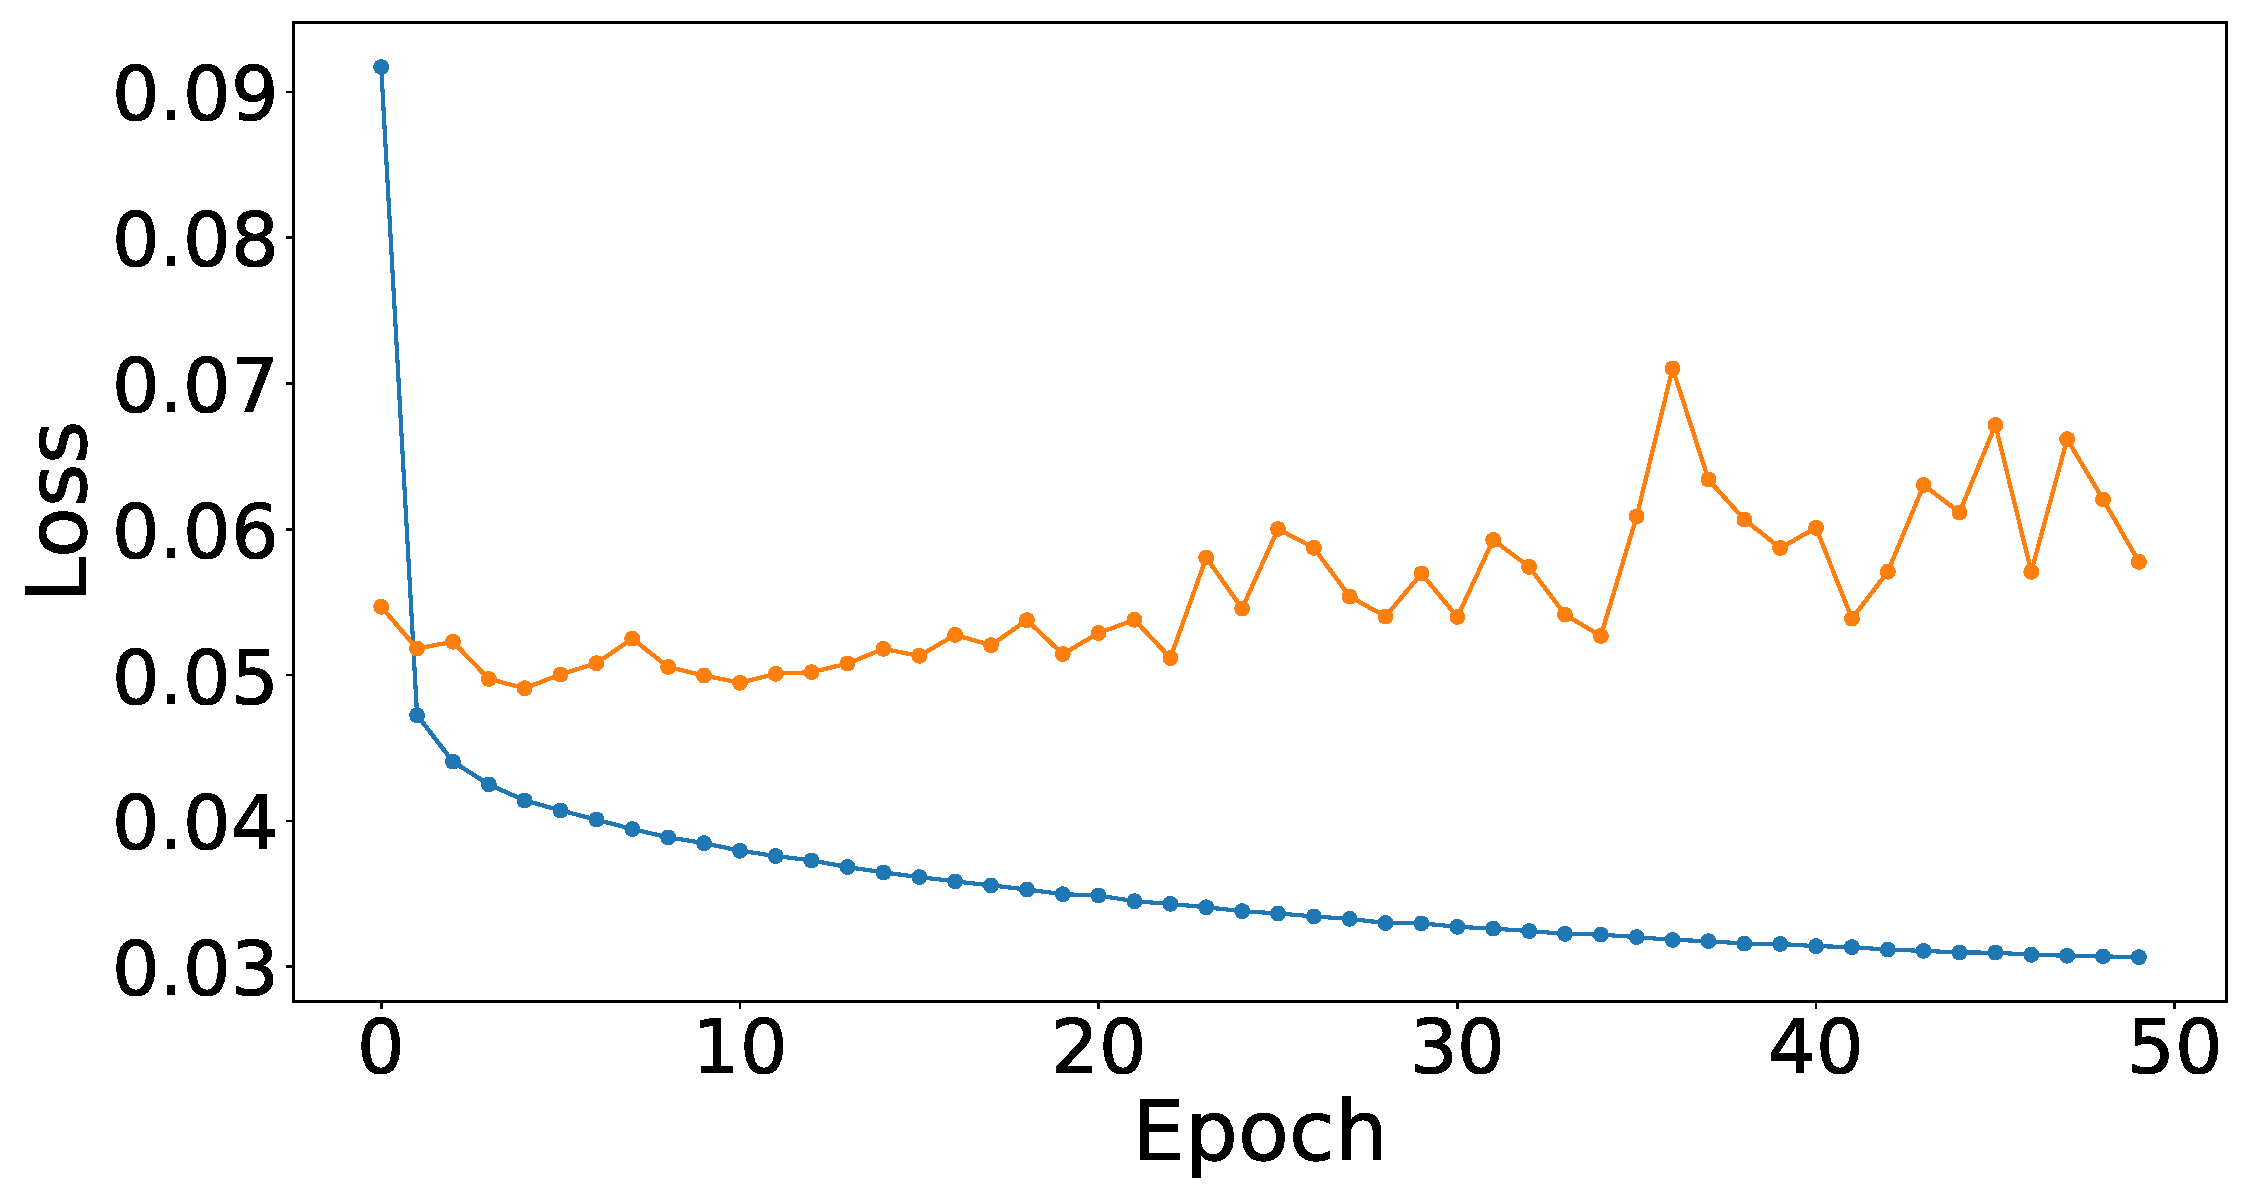
\includegraphics[width=\linewidth]{Figures/ncf_training_1_sample.pdf} % Adjust the width as needed
        \caption{Model 1: ratings only}
        \label{fig:model1_sample} 
    \end{subfigure}
    \hfill
    \begin{subfigure}{0.49\textwidth}
        \centering
        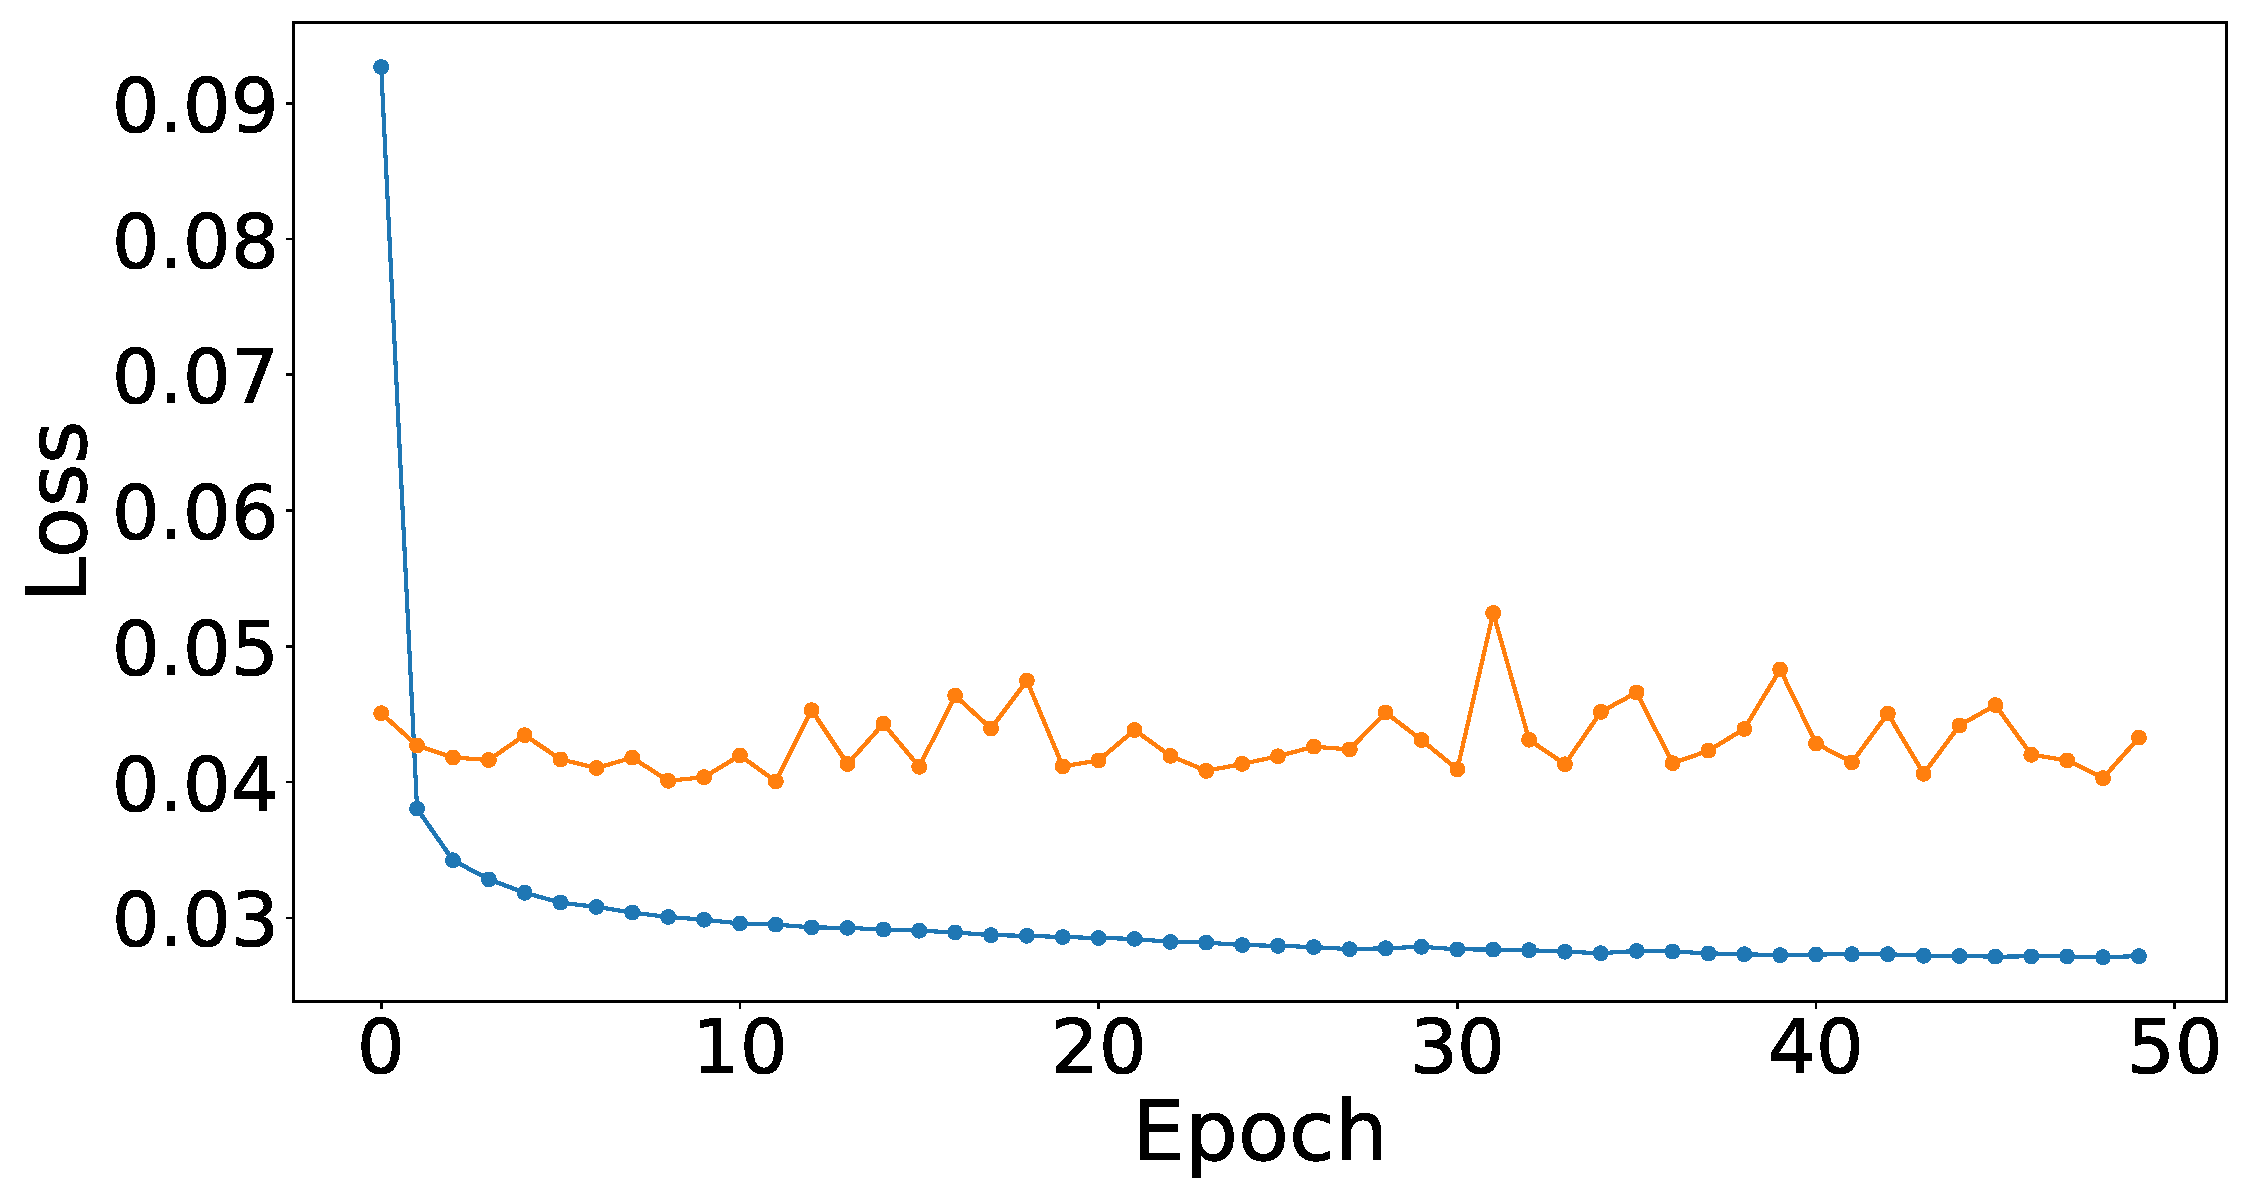
\includegraphics[width=\linewidth]{Figures/ncf_training_2_sample.pdf} % Adjust the width as needed
        \caption{Model 2: ratings and review texts}
        \label{fig:model2_sample}
    \end{subfigure}
    \hfill
    \begin{subfigure}{0.49\textwidth}
        \centering
        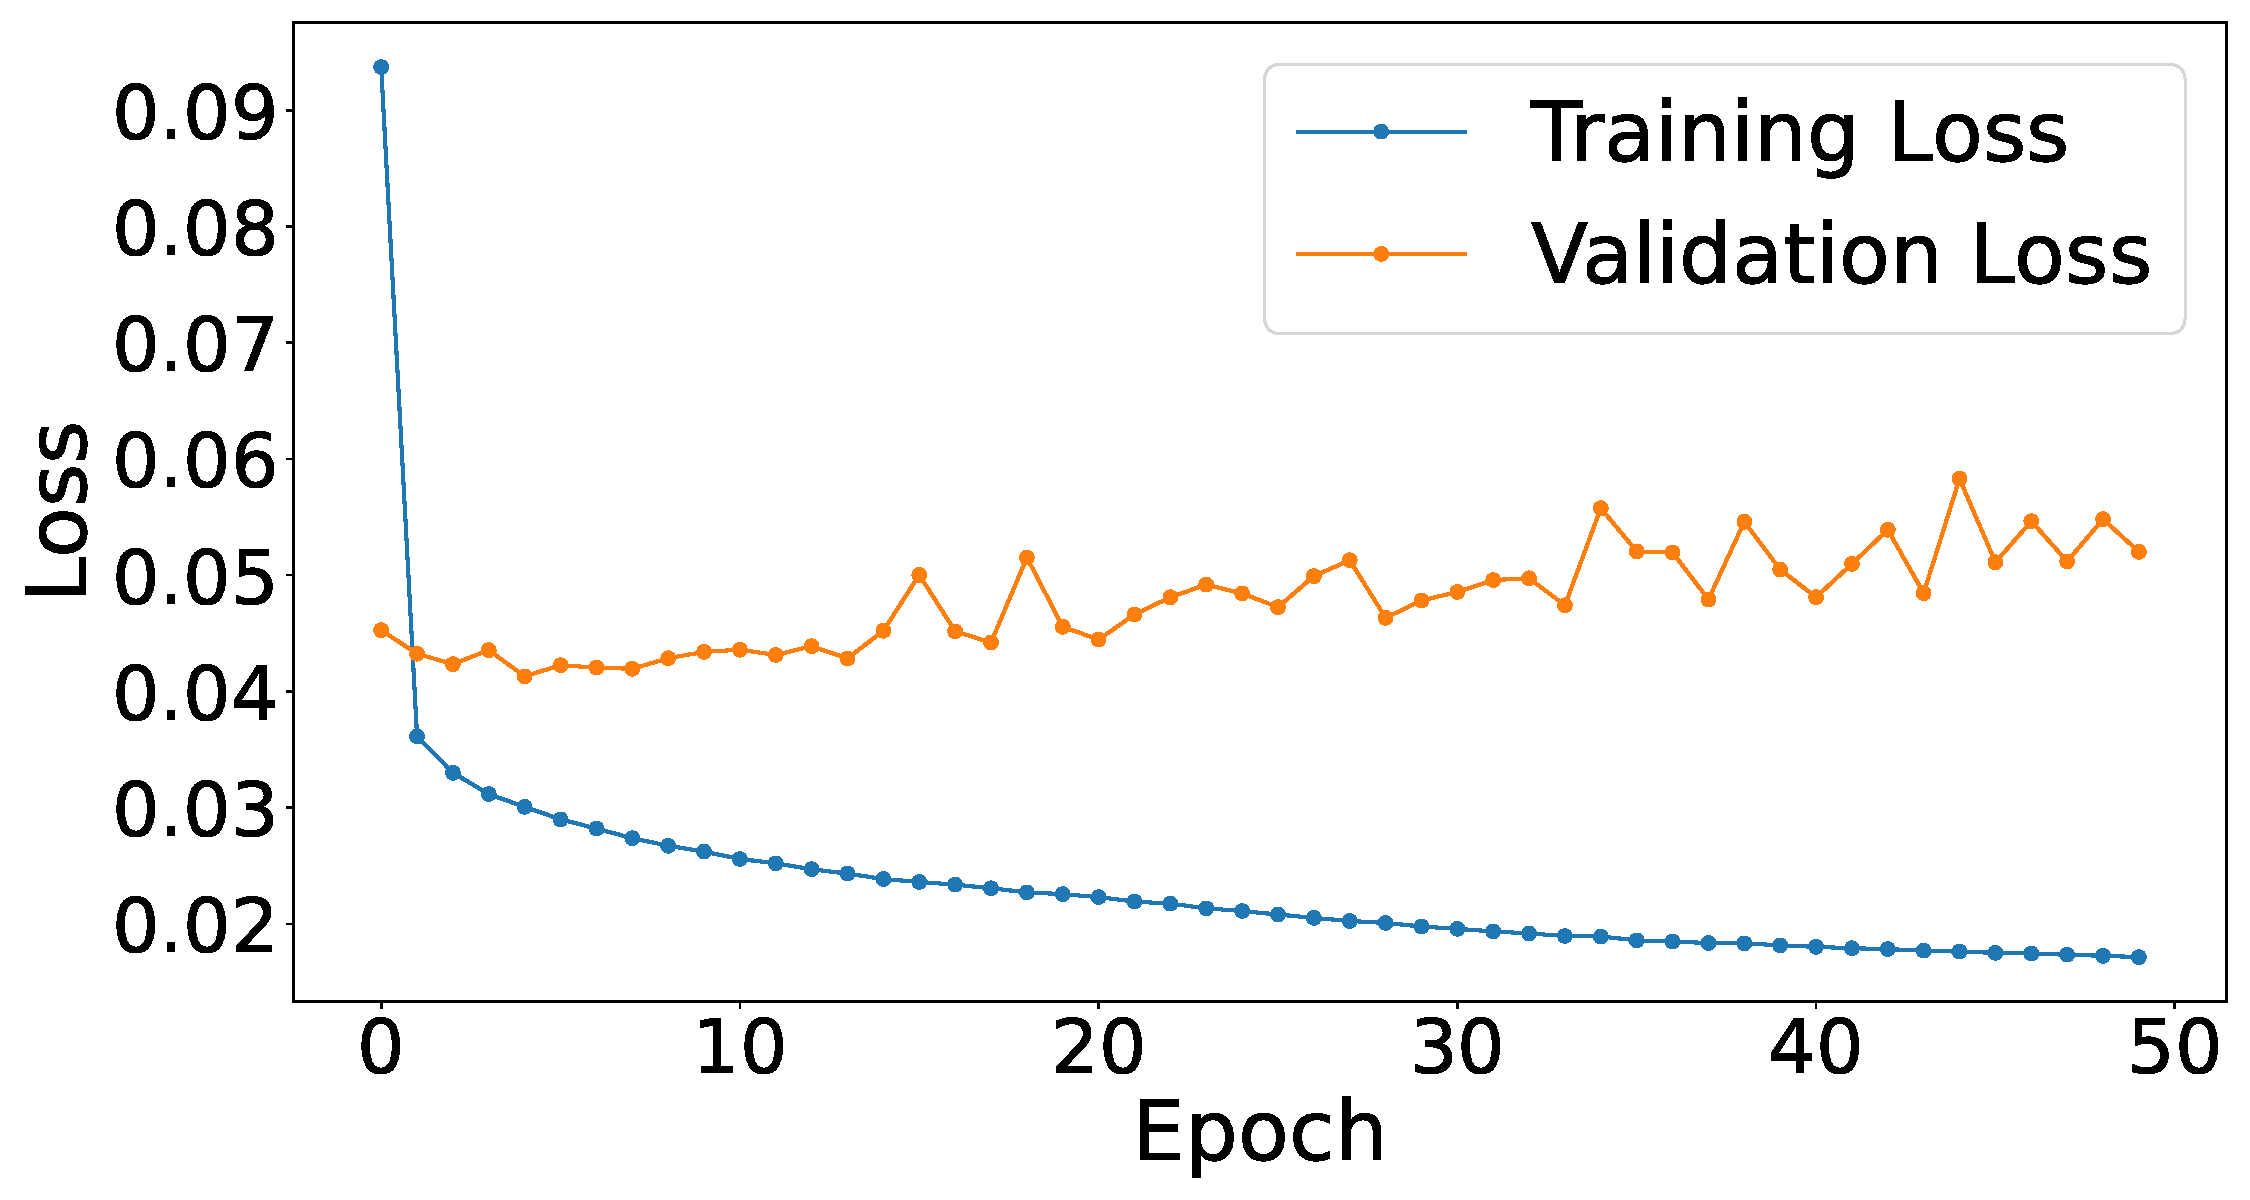
\includegraphics[width=\linewidth]{Figures/ncf_training_3_sample.pdf} % Adjust the width as needed
        \caption{Model 3: ratings, review texts and sentiments}
        \label{fig:model3_sample}
    \end{subfigure}
    \caption{Training and validation curves for example combination of hyperparameters for all three NCF models.}
    \label{train_val_curves_sample}
\end{figure}


\begin{table}[h]
    \centering
    \begin{tabular}{|p{6cm}|p{3cm}|}
    \hline
    \textbf{Hyperparameter} & \textbf{Value}  \\
    \hline
    Learning Rate & 0.001 \\
    Epochs & 50 \\
    Batch Size & 32 \\
    Number of Layers & 6 \\
    Number of Units in First Layer & 512\\
    Dropout Rate & 0.0 \\
    Optimiser & Adam \\
    L2 Regularisation & 0.001 \\
    \hline
    \end{tabular}
    \caption{Example combination of hyperparameters for NCF models.}
    \label{tab:hyper_sample}
    \end{table}

% createa table with columns: model, hyperparameter, value. Model must be multirow. Have three models


    \begin{table}[h]
        \centering
        \begin{tabular}{|p{3cm}|p{6cm}|p{3cm}|}
        \hline
        \textbf{Model} & \textbf{Hyperparameter} & \textbf{Value}  \\
        \hline
        \multirow{8}{*}{Model 1} & Learning Rate & 0.001 \\
        & Epochs & 50 \\
        & Batch Size & 128 \\
        & Number of Layers & 2 \\
        & Number of Units in First Layer & 512\\
        & Dropout Rate & 0.5 \\
        & Optimiser & Adam \\
        & L2 Regularisation & 0.01 \\
        \hline
        \multirow{8}{*}{Model 2} & Learning Rate & 0.001 \\
        & Epochs & 50 \\
        & Batch Size & 128 \\
        & Number of Layers & 3 \\
        & Number of Units in First Layer & 512 \\
        & Dropout Rate & 0.5 \\
        & Optimiser & Adam \\
        & L2 Regularisation & 0.01 \\
        \hline
        \multirow{8}{*}{Model 3} & Learning Rate & 0.001 \\
        & Epochs & 50 \\
        & Batch Size & 128 \\
        & Number of Layers & 3 \\
        & Number of Units in First Layer & 512 \\
        & Dropout Rate & 0.5 \\
        & Optimiser & Adam \\
        & L2 Regularisation & 0.01 \\
        \hline
        \end{tabular}
        \caption{Final combination of hyperparameters for NCF models.}
        \label{tab:hyper_final}
    \end{table}


For Figure \ref{train_val_curves_sample}, we observe the training loss decreasing over each epoch for all models, indicating that the models are learning the patterns in the data and improving their predictive capabilities. The validation loss, however, appears to show a general increasing trend for Figures \ref{fig:model1_sample} and \ref{fig:model3_sample}. This is likely due to the model's inability to generalise well to unseen data, suggesting that the models may be overfitting the training data. Additionally, the training and validation curves are also far apart (and increasing in distance), suggesting that the models are not generalising well to unseen data \cite{diaz2017effective}. There are seeveral possible reasons as to why this is the case. Firstly, our model architecture could be too complex given the dataset. It may be memorising the training data. A simple fix would be to simplify the model. This can be achieved by reducing the hidden layers or units, or applying regularisation \cite{bergstra2011algorithms}. Table \ref{tab:hyper_sample}, indicates that there was no dropout rate applied (0.0), as well as a relatively high number of hidden layers (6). This combination of hyperparameters may be leading the model to not generalise well to unseen data and overfit the training data. 

\begin{figure}[h]
    \centering
    \begin{subfigure}{0.49\textwidth}
        \centering
        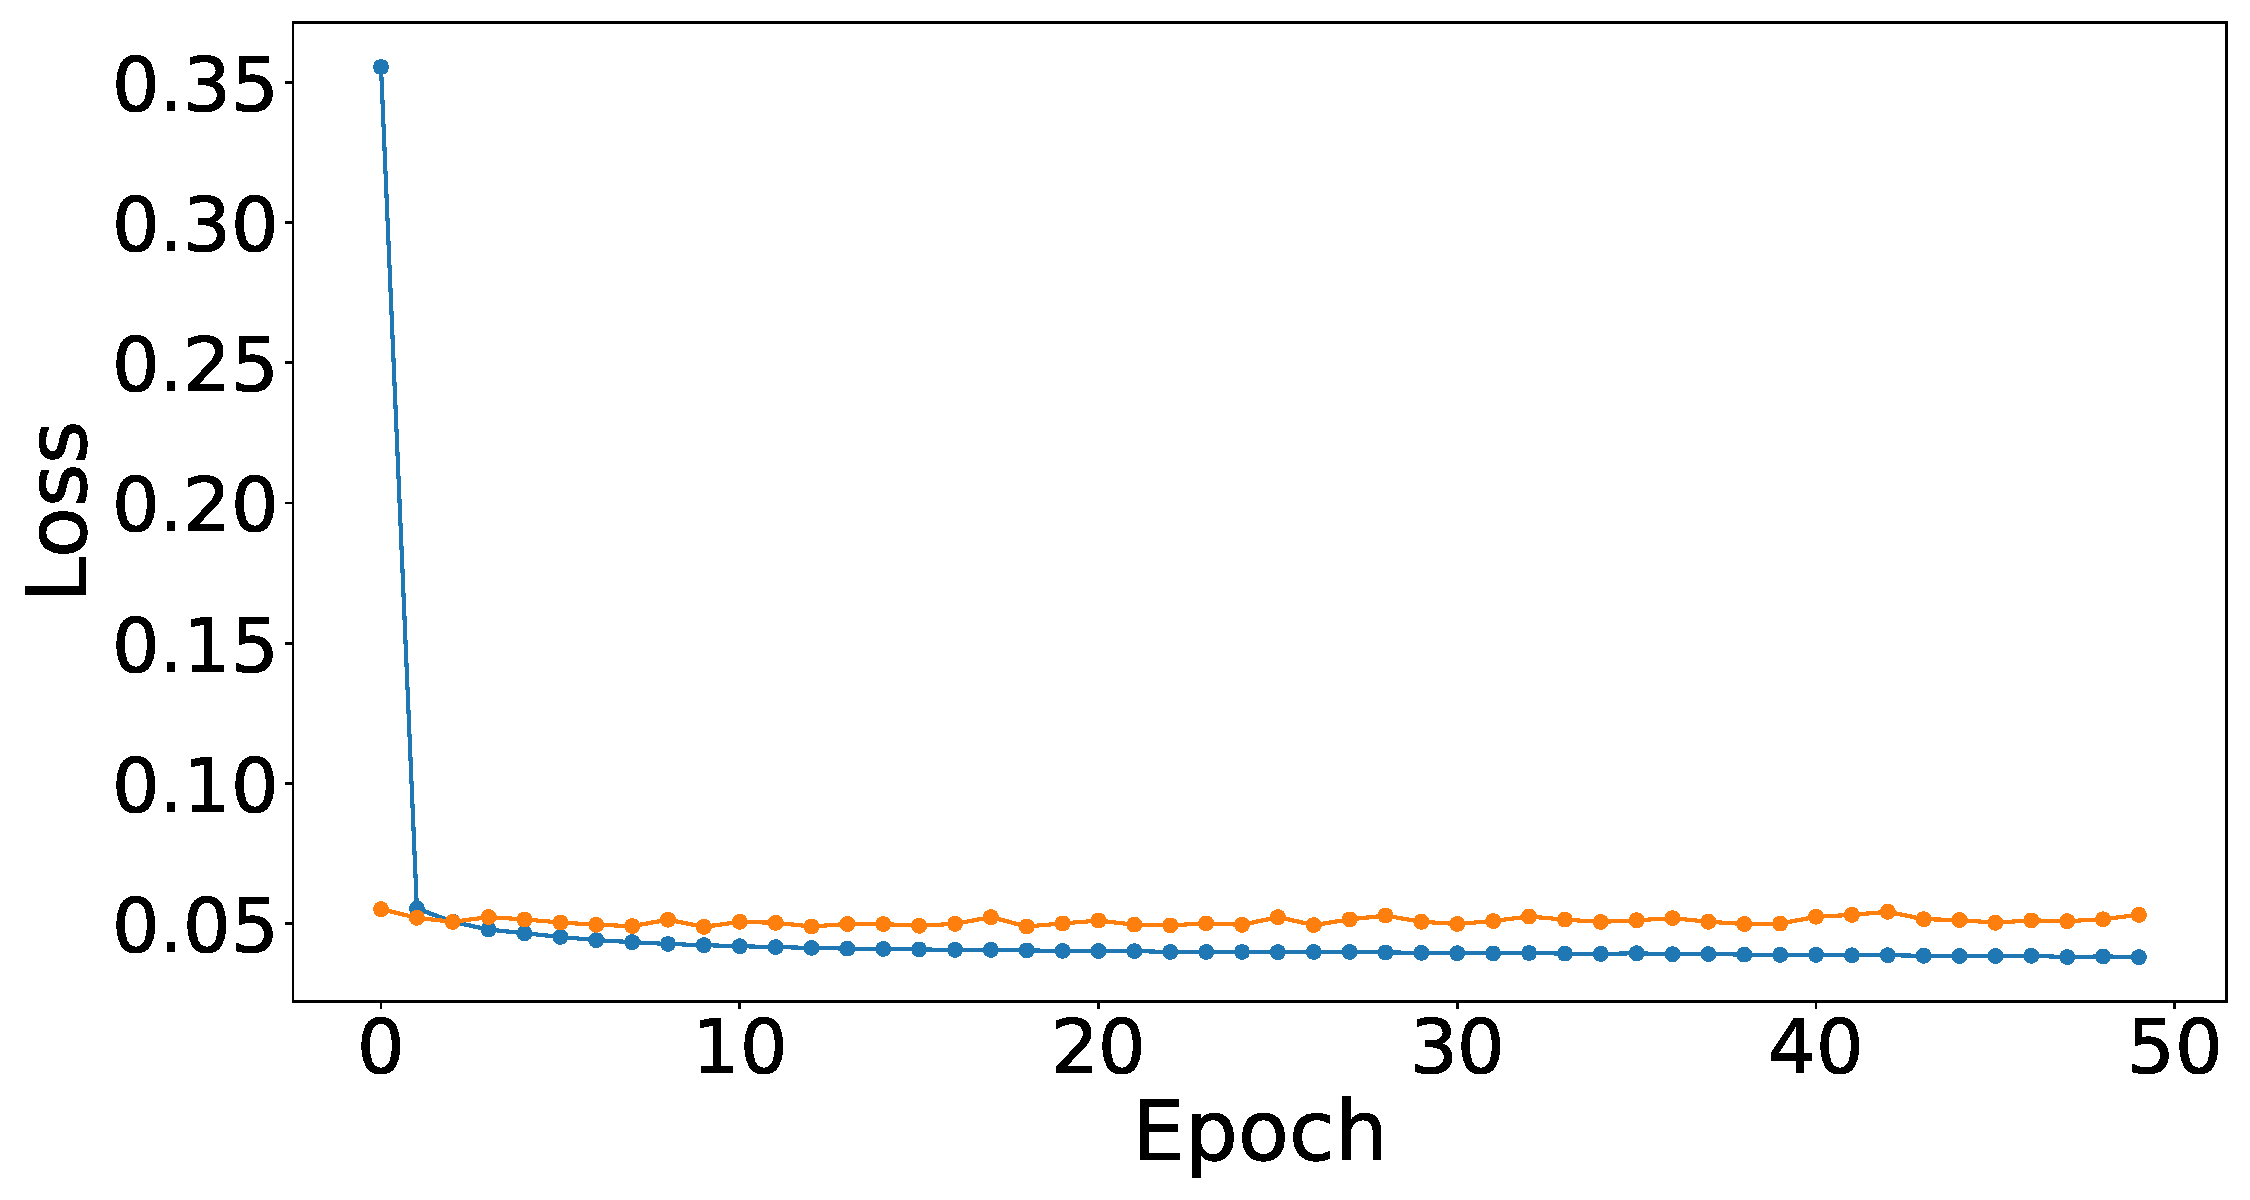
\includegraphics[width=\linewidth]{Figures/ncf_training_1.pdf} % Adjust the width as needed
        \caption{Model 1: ratings only}
        \label{fig:model1} 
    \end{subfigure}
    \hfill
    \begin{subfigure}{0.49\textwidth}
        \centering
        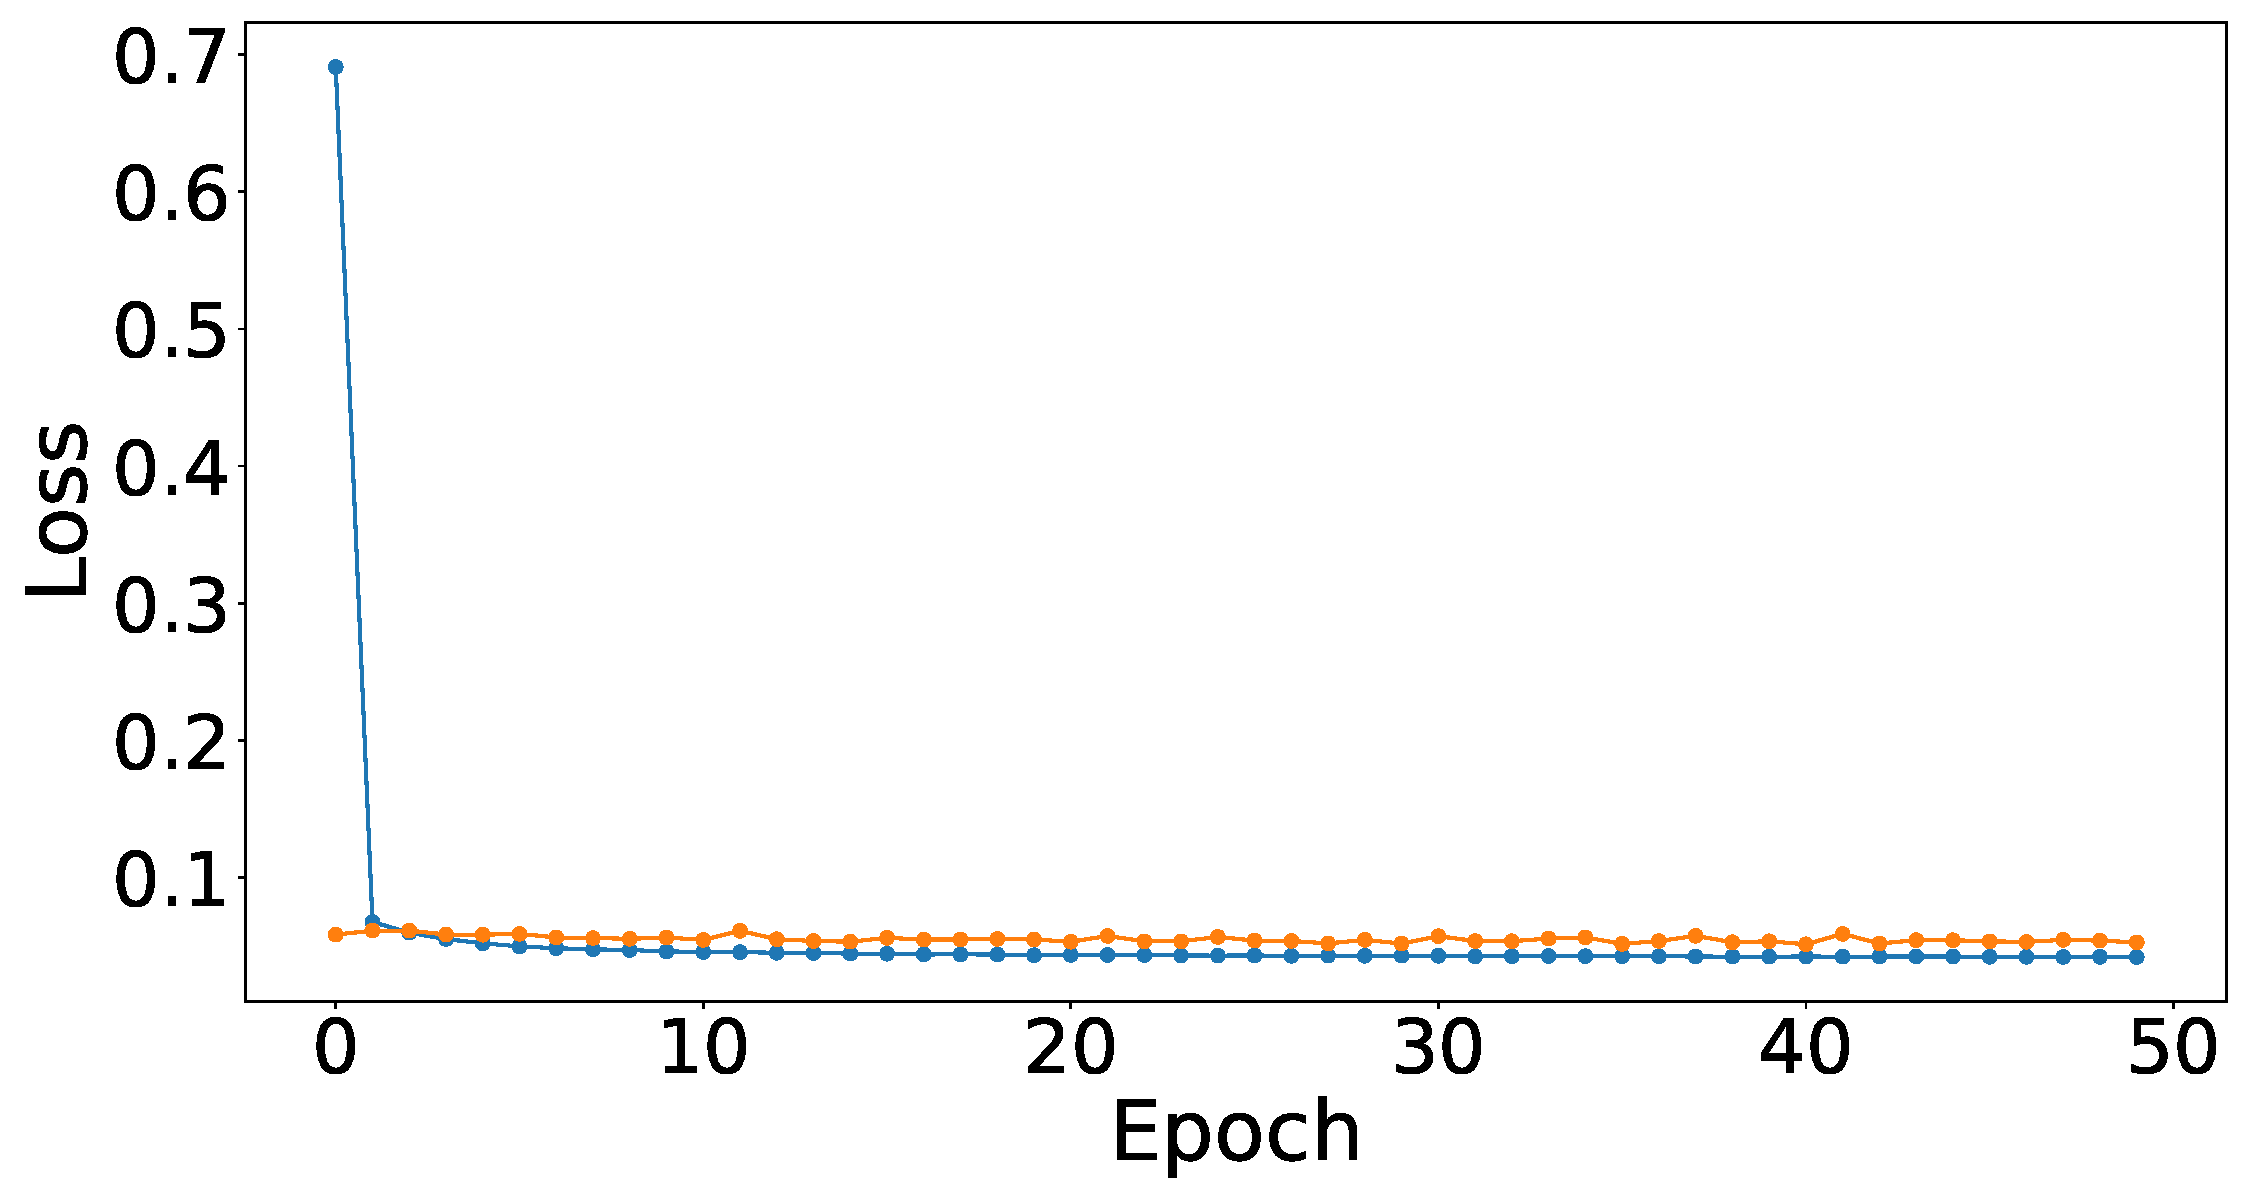
\includegraphics[width=\linewidth]{Figures/ncf_training_2.pdf} % Adjust the width as needed
        \caption{Model 2: ratings and review texts}
        \label{fig:model2}
    \end{subfigure}
    \hfill
    \begin{subfigure}{0.49\textwidth}
        \centering
        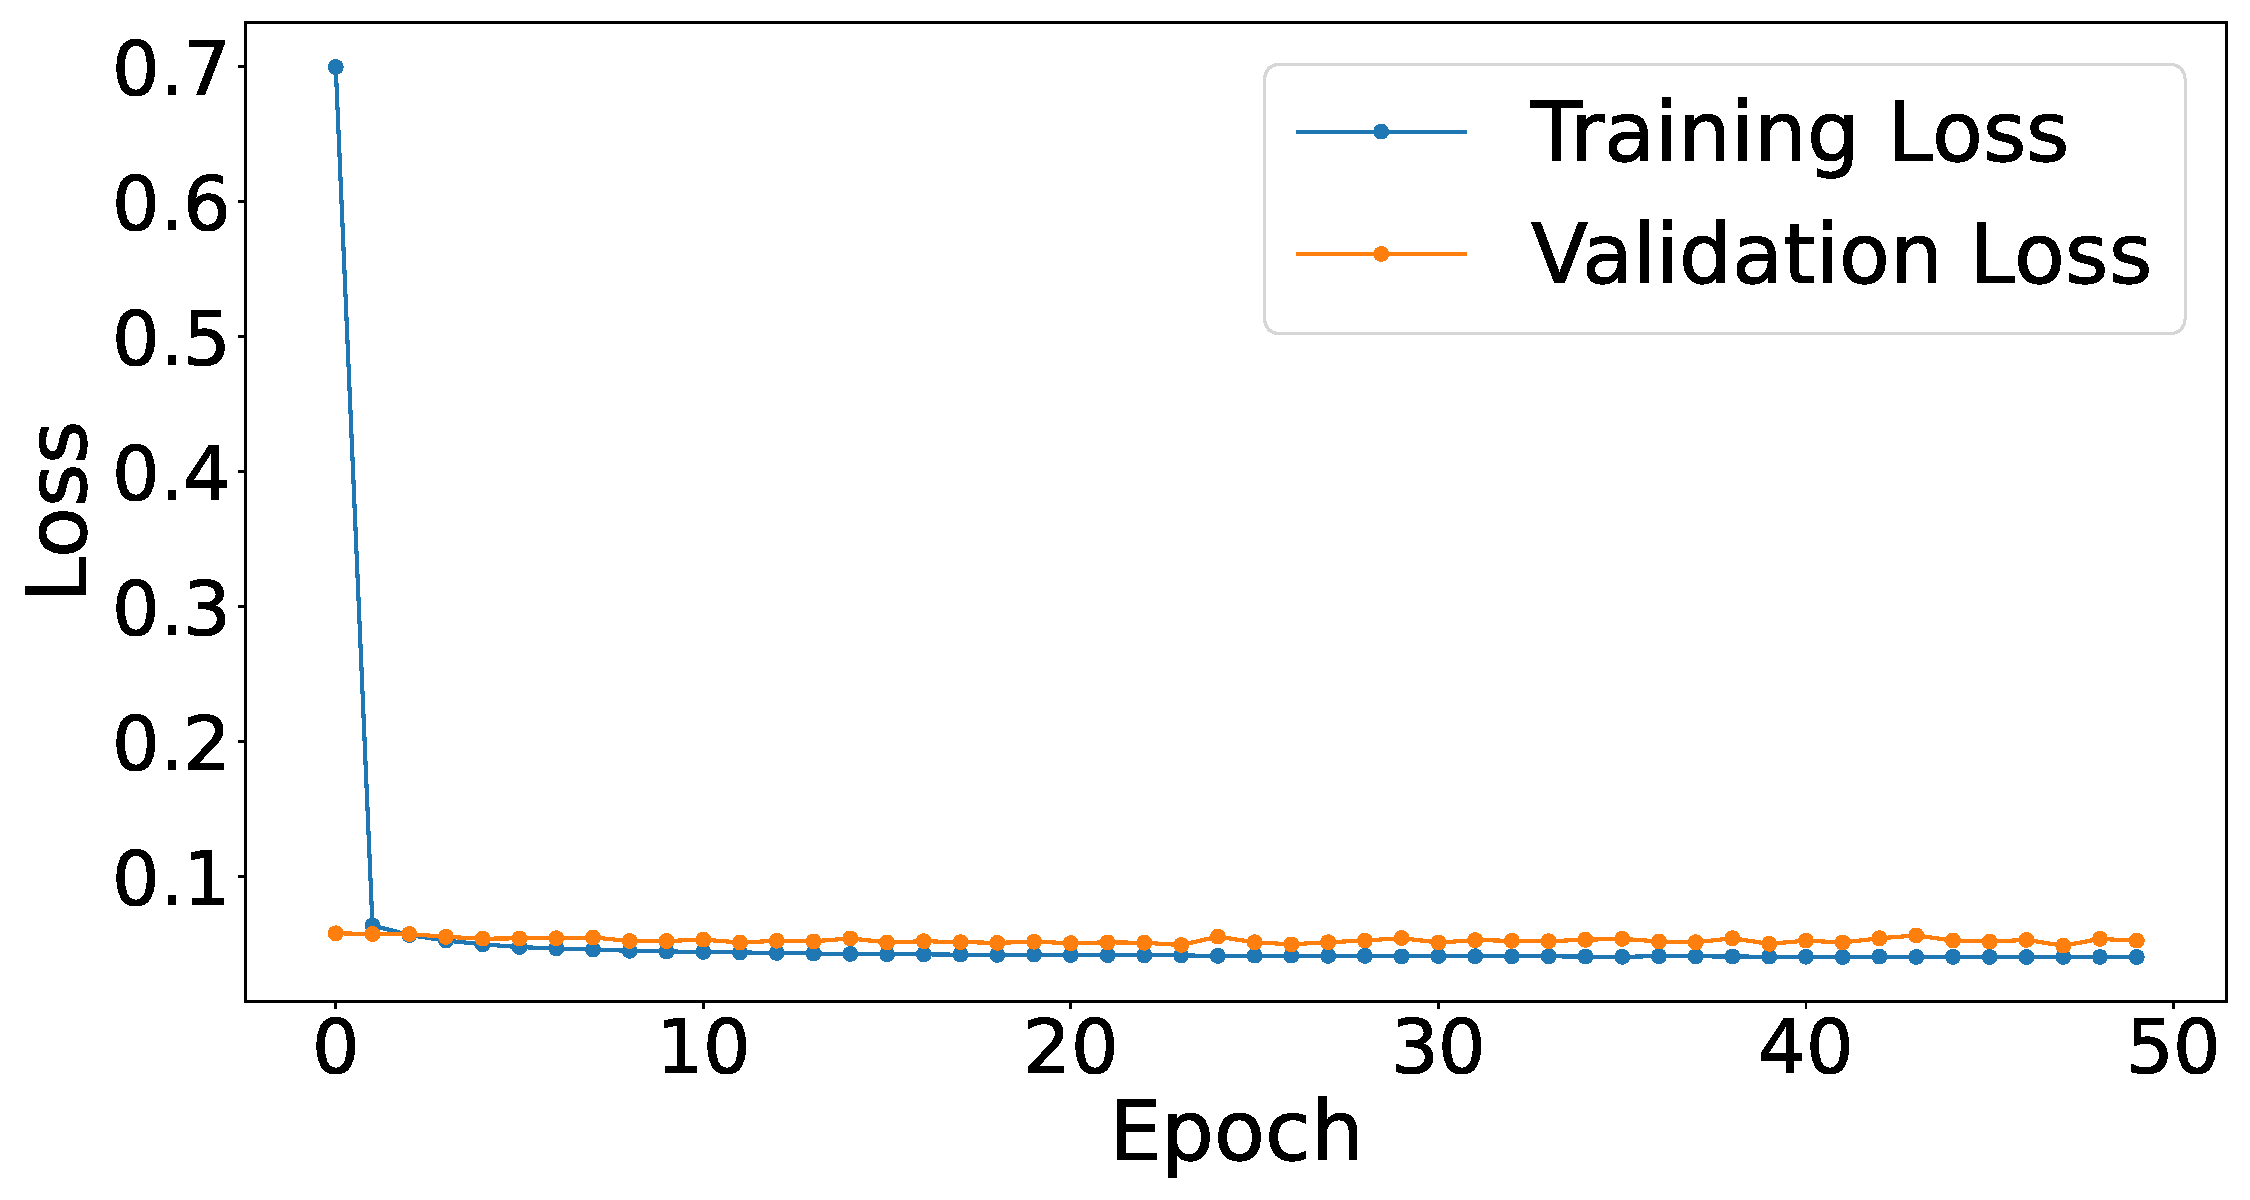
\includegraphics[width=\linewidth]{Figures/ncf_training_3.pdf} % Adjust the width as needed
        \caption{Model 3: ratings, review text and sentiments}
        \label{fig:model3}
    \end{subfigure}
    \caption{Training and validation curves for the best combination of hyperparameters from the set for all three NCF models.}
    \label{fig:train_val curves final}
\end{figure}


The training and validation curves for the best hyperparameter combinations for each of the three NCF models are shown in Figure \ref{fig:train_val curves final}. The curves indicate that all the models are learning the patterns in the data effectively and are performing well on both the training and validation datasets. This is illustrated by both the training and validation curves decreasing for all the models in Figure \ref{fig:train_val curves final}. Similarly, the training and validation curves are close to each other, indicating that the models are generalising well to unseen data. The curves are also smooth, suggesting that the models are converging well and not experiencing convergence problems \cite{bergstra2011algorithms}. Overall, the training and validation curves suggest that the models are learning the patterns in the data effectively and are performing well on both the training and validation datasets. Table \ref{tab:hyper_final} displays the final combinations of hyperparameters for each of the three models. As previously mentioned, these combinations of hyperparameters were selected based on the best performance on the validation dataset. 


\subsection{Summary}
\label{sec:4 Summary for NCF}

This section began by providing a overview of the workings of and implementation of our NCF models. Effectively, the NCF model comprises multiple layers (see Figure \ref{fig:neural_network}), each serving a unique purpose in the model process. The input feature layer accepts user and item feature vectors, $\mathbf{v}_u^U$ and $\mathbf{v}_i^I$, respectively. From here, the embedding layer transforms these user and item vectors into user and item embeddings respectively. Subsequently, the user and item embeddings are concatenated to form the input vector, $\mathbf{x}_{ui}$, which serves as the input vector to the NCF layer. Additionally, for model 2 and 3 we discussed how we would extend the input vector $\mathbf{x}_{ui}$ to include the review text embeddings and sentiment embeddings, respectively. This concatenation results in a combined feature vector that captures the latent features and relationships between users, items, and the augmented features (embeddings). The concatenated input vector then traverses through multiple NCF layers, each leveraging rectified linear units (ReLU) as activation functions. The final output layer predicts the rating $\hat{y}_{u i}$ for a user $u$ for item $i$. 

We also delved into the training process, where we optimise the model parameters ($\boldsymbol{\Theta}_f$) which includes the weights and biases of the neural network and the user and item embeddings. For model 2 and 3, we would also include the review text embedding as a model parameter, and this too will be optimised in the training process. These parameters are optimised so as to minimise the regularised mean square error loss function (Equation \ref{eq:mse}). Additionally, we discussed in detail the hyperparameter tuning process and results. Hyperparameter tuning was done using the validation data and using a grid search technique. The best combination of hyperparameters (from the pool of options chosen) was used found for each model and used to create the final specification of that model. We conclude this section by outlining the three respective NCF models built and their architectures. Note, the optimal hyperparameters for all three models were summarised in Table \ref{tab:hyper_final}.
\\
\\
\textbf{Model 1: Ratings Only}

Model 1 is the simplest of the three models, utilising only numerical ratings from the users  to make predictions. The neural network model architecture (or NCF layers) are composed of two hidden layers, each with 512 units. The dropout rate is set to 0.5, and the L2 regularisation term is set to 0.001. The model is trained for 50 epochs with a batch size of 128. The learning rate is set to 0.001, and the optimiser used is Adam. The final output layer predicts the rating for a user-item pair. The hyperparameters for Model 1 are shown in Table \ref{tab:hyper_final}. The achieved validation loss for this model is 0.050.
\\
\\
\textbf{Model 2: Ratings Only}

Model 2 extends Model 1 by incorporating user review text into the model. The neural network model architecture (or NCF layers) are composed of three hidden layers, each with 512 units. The dropout rate is set to 0.5, and the L2 regularisation term is set to 0.01. The model is trained for 50 epochs with a batch size of 128. The learning rate is set to 0.001, and the optimiser used is Adam. Similar to model 1, the final output layer predicts the rating for a user-item pair. The hyperparameters for model 2 are shown in Table \ref{tab:hyper_final}. The achieved validation loss for this model is 0.043. 
\\
\\
\textbf{Model 3: Ratings, Review Text and Sentiments}

Model 3 is the most complex of the three models, incorporating user review text and sentiments into the model. The neural network model architecture (or NCF layers) are composed of three hidden layers, each with 512 units. The dropout rate is set to 0.5, and the L2 regularisation term is set to 0.01. The model is trained for 50 epochs with a batch size of 128. The learning rate is set to 0.001, and the optimiser used is Adam. The final output layer predicts the rating for a user-item pair. The hyperparameters for model 3 are shown in Table \ref{tab:hyper_final}. The achieved validation loss for this model is 0.043.


\section{Benchmark Models}
\label{sec:4 Benchmark Models}

In our analysis and development of NCF, which serves as the cornerstone of this thesis, the imperative now lies in comparing its performance and discerning whether the integration of deep learning approaches actually brings about substantial improvements in collaborative filtering. To facilitate this comparison, we introduce three additional benchmark models more aligned and often associated with conventional collaborative filtering methodologies. These models are constructed to generate both rating predictions and Top-N ranked lists (like the NCF models). By discussing and applying these models we can directly facilitate the comparison of a deep-learning recommender approach those more traditional techniques. The ensuing subsections looks into the technical details and specifications of these benchmark models, providing a comprehensive understanding of their design and functionality.


\subsection{Non-Negative Matrix Factorisation}
\label{subsec:4 Non-Negative Matrix Factorisation}

As mentioned in Section \ref{sec:2 Collaborative Filtering}, matrix factorisation has emerged as one of the most successful implementations of collaborative filtering, particularly within latent factor models and the model-based framework of collaborative filtering \cite{koren2009collaborative}. The fundamental concept of matrix factorisation involves representing both users and items through vectors of factors derived from item-rating interactions \cite{koren2009collaborative}. This method gained popularity post the Netflix Competition for its commendable scalability coupled with predictive accuracy. 

Non-Negative Matrix Factorisation (NMF) is a variant of matrix factorisation that has been widely applied in collaborative filtering tasks \cite{lee2000algorithms}. NMF is a dimensionality reduction technique that decomposes a given matrix into two non-negative matrices, $\mathbf{W}$ and $\mathbf{H}$, where $\mathbf{W}$ can represent the user-feature matrix, where each row corresponds to a user and the columns capture latent features, whilst $\mathbf{H}$ can represent the item-feature matrix, where each column corresponds to an item and the rows capture latent features. Furthermore, NMF imposes non-negativity constraints on these factor matrices, so as to ensure that the derived features are inherently non-negative, promoting interpretability and facilitating meaningful representations in diverse applications \cite{koren2009matrix}. This particular matrixfactorisation method was chosen due to its simplicity, interpretability, and effectiveness in capturing latent features within the data (\cite{koren2009matrix}; \cite{lee2000algorithms}).


\subsubsection{Algorithm Formulation and Summary}
\label{subsubsec:4 Algorithm Formulation MF}

Specifically, a matrix factorisation model establishes a mapping of users and items to a shared latent factor space of dimensionality $f$ \cite{}. This mapping enables the modelling of user-item interactions as inner products within this factor space. For NMF, each item $i$ is represented by a vector $q_i \in \mathbb{R}^f$, and each user $u$ is associated with a vector $\mathbf{p}_u \in \mathbb{R}^f$. For a given item $i$, the elements of $\mathbf{q}_i$ measure the extent to which the item possesses those factors, with higher values indicating a stronger association between the item and the factor \cite{}. Similarly, for a given user $u$, the elements of $\mathbf{p}_u$ measure the extent of interest the user has in items that are high on the corresponding factors, again, higher values indicate a stronger association between the user and the factor. The dot product $\mathbf{q}_i^T \mathbf{p}_u$ captures the interaction between user $u$ and item $i$, approximating the user's rating $\left(r_{u i}\right)$ for item $i$ \cite{}. . By extension, $\mathbf{Q}$ and $\mathbf{P}$ represent the factor matrices for all items and users, respectively. That is, these matrices are are composed of the factor vectors $\mathbf{q}_i$ and $\mathbf{p}_u$ as their columns, respectively. Thus, we can estimate the user's rating for an item using Equation \ref{eq:MF rating prediction}.

\begin{equation}
    \hat{r}_{u i} = \mathbf{Q}_i^T \mathbf{P}_u
    \label{eq:MF rating prediction}
    \end{equation}


The primary challenge for NMF lies in computing the factor matrices $\mathbf{Q}$ and $\mathbf{P}$ for all items and users. This is achieved by minimising some objective function using an optimisation algorithm. The objective function is typically the squared error between the observed ratings and the predicted ratings. The objective function for NMF can be formulated as shown in Equation \ref{eq:MF objective function}.

\begin{equation}
    \label{eq:MF objective function}
    \min_{Q, P} \sum_{(u, i) \in \kappa} \left(r_{ui} - \mathbf{Q}^T_i \mathbf{P}_u\right)^2
\end{equation}

In Equation \ref{eq:MF objective function}, $\kappa$ represents the set of observed user-item ratings. $\mathbf{Q}$ is the matrix containing the latent factors associated with items, whilst $\mathbf{P}$ is the matrix containing the latent factors associated with users. As such, $\mathbf{Q}^T_i$ represents the $i$-th column of the transpose of matrix $\mathbf{Q}$, corresponding to the latent factors for item $i$ (i.e., $\mathbf{q}_i$). Similarly, $\mathbf{P}_u$ represents the $u$-th row of matrix $\mathbf{P}$, corresponding to the latent factors for user $u$ (i.e., $\mathbf{p}_u$). Additionally, $r_{ui}$ denotes the observed rating for user $u$ on item $i$. 

The goal in NMF, is to learn the factor vectors $\mathbf{Q}$ and $\mathbf{P}$ that minimise the squared error between the observed ratings ($r_{ui}$) and the predicted ratings ($\hat{r}_{ui}$). To achieve this, an optimisation algorithm is used with training data to update the factor vectors $\mathbf{Q}$ and $\mathbf{P}$ iteratively. Specifically, the factor matrices $\mathbf{Q}$ and $\mathbf{P}$ are updated using the gradient of the objective function with respect to the factor matrices. The gradient provides information on the direction and magnitude of the steepest ascent in the objective function. By moving against the gradient, the factor matrices are updated to minimise the objective function. To this end, the optimisation algorithm iteratively updates the factor vectors $\mathbf{Q}$ and $\mathbf{P}$ to minimise the objective function. The algorithm continues to update the factor matrices until the objective function converges to a minimum or a predefined stopping criterion is met. The factor matrices $\mathbf{Q}$ and $\mathbf{P}$ capture the latent features of the users and items, respectively. Effecitvely, once this mapping is achieved, the recommender system can estimate user ratings for any item using Equation \ref{eq:MF rating prediction}. For this thesis, to minimise equation \ref{eq:regularised error MF}, there are two popular optimisation algorithms - SGD and alternating least squares\footnote{}. We opted for SGD due to its popularity in similar research papers (\cite{rendle2020neural}; \cite{lee2000algorithms}) where NMF models were developed. 

An additional area of concern is the inherent sparsity in the user-item ratings matrix (see Section \ref{subsec:2 Sparsity}). Addressing only observed entries risks overfitting \cite{koren2009matrix}, particularly in scenarios with a high proportion of missing values. To mitigate this, some approaches (\cite{paterek2007improving};\cite{takacs2007major}) propose modeling observed ratings directly while preventing overfitting through regularisation. This in fact the approach taken for this building this benchmark model. The system minimises the regularised squared error on the set of known ratings. As such, the updated objective function for NMF with regularisation can be formulated as shown in Equation \ref{eq:regularised error MF}.

    \begin{equation}
        \min_{Q, P} \sum_{(u, i) \in \kappa} \left(r_{ui} - \mathbf{Q}^T_i \mathbf{Q}_u\right)^2 + \lambda \left(\|Q\|^2 + \|P\|^2\right)
        \label{eq:regularised error MF}
    \end{equation}
    

In Equation \ref{eq:regularised error MF}, $\mathbf{Q}$ and $\mathbf{P}$ (as well as $\mathbf{Q}^T_i$ and $\mathbf{P}_u$) are defined as previously mentioned. The parameter $\lambda$ is the regularisation parameter that controls the strength of the regularisation term and is usually determined by cross-validation \cite{koren2009matrix}. The regularisation term penalises the sum of the squared elements of the factor matrices $\mathbf{Q}$ and $\mathbf{P}$. The regularisation term discourages the factor vectors from becoming too large, thereby preventing overfitting and improving the generalisation capabilities of the model \cite{koren2009matrix}. Once the factor matrices $\mathbf{Q}$ and $\mathbf{P}$ have been learned, the model can predict the rating for any user-item pair using Equation \ref{eq:MF rating prediction}. To evaluate the performance of the NMF model, we assess how accurate the rating predictions are for unseen data, using the test dataset. 

We provide the steps for NMF in Algorithm \ref{algo:MF}. In summary, the algorithm begins by initialising the factor matrices $\mathbf{Q}$ and $\mathbf{P}$ with random values. The algorithm then iteratively updates the factor matrices using the gradient of the objective function with respect to the factor matrices. The algorithm continues to update the factor matrices until the objective function converges to a minimum or a predefined stopping criterion is met. The factor matrices $\mathbf{Q}$ and $\mathbf{P}$ capture the latent features of the users and items, respectively. Once the factor matrices have been learned, the model can predict the rating for any user-item pair using Equation \ref{eq:MF rating prediction}. The algorithm outputs the predicted ratings for the test dataset, which can be used to evaluate the models ability to correctly predict ratings for users. Subsequently, we can rank every predicted rating for each user and provide a list of top-N recommendations for each user, and hence evaluate this. 

\begin{algorithm}
    \caption{Non-Negative Matrix Factorisation Algorithm Summary}
    \begin{algorithmic}[1]
      \State \textbf{Initialisation}
       \newline \quad Begin with the initial user and item matrices, $P$ and $Q$, containing non-negative values.
       \newline \quad Set the number of latent factors, $f$, representing the dimensionality of the latent factor space.
    
      \State \textbf{Factorisation}
       \newline \quad Iteratively update the factor matrices $P$ and $Q$ by minimising the squared error on the set of known ratings.
       \newline \quad Utilise optimisation techniques such as stochastic gradient descent to achieve convergence.
    
      \State \textbf{Regularisation}
       \newline \quad Optionally introduce regularisation terms to the objective function to prevent overfitting.
       \newline \quad Adjust the regularisation parameter ($\lambda$) through cross-validation to optimise model performance.
        
      \State \textbf{Optimization}
       \newline \quad Employ cross-validation to determine optimal parameter values and ensure model robustness.
    
      \State \textbf{Prediction Accuracy}
       \newline \quad Assess the model's performance by comparing predicted ratings ($\hat{y}_{u i}$) against actual ratings, consistent with the evaluation process for Neural Collaborative Filtering.
    
      \State \textbf{Top-N Evaluation}
       \newline \quad Evaluate the model's ability to generate Top-N recommendations by ranking predicted ratings for unrated items, consistent with the evaluation process for Neural Collaborative Filtering.
    \end{algorithmic}
    \end{algorithm}
    
The NMF model was built in Python from fundamentals. NMF has several hyperparameters that need to be set when training the model. These hyperparameters include the number of latent factors ($k$), the learning rate, the regularisation parameter ($\lambda$), and the number of epochs. The learning rate is the same as previously defined in NCF. Epochs in the context of NMF, refers to the number of iterations over the entire dataset during training. The regularisation parameter ($\lambda$) is a hyperparameter that controls the strength of the regularisation term in the objective function. The number of latent factors ($k$) is the number of latent factors that the model will learn to represent the data. Specifically, $k$ is the number of latent factors that we assume exist in the data \cite{}. These latent factors are learned during the factorisation process and are represented by the columns of matrices $\mathbf{Q}$ and $\mathbf{P}$. Effectively, $k$ determines the number of dimensions in which the user and item vectors are represented. That is, the matrix $\mathbf{Q}$ has dimensions $m \times k$, where $m$ is the number of items, and the matrix $\mathbf{P}$ has dimensions $n \times k$, where $n$ is the number of users \cite{}. Thus, the choice of $k$ determines the number of latent factors that the model will learn to represent the data. A higher value of $k$ allows the model to capture more complex patterns in the data but may also increase the risk of overfitting. Conversely, a lower value of $k$ results in a more simplified representation of the data but may lead to underfitting \cite{}. To determine the optimal hyperparameters for the NMF model, a grid search was performed over a range of hyperparameters, albeit, the number of combinations was limited due to the computational tax incurred in running the developed NMF model. Thus, we limited the number of combinations for NMF for this thesis. Table \ref{hyper_params_mf} displays the hyperparameter combinations for the NMF model.



\begin{table}[h]
    \centering
    \begin{tabular}{|p{5cm}|p{7cm}|p{3.5cm}|}
    \hline
    \textbf{Hyperparameter} & \textbf{Description}  & \textbf{Combinations} \\
    \hline
    Number of Latent Factors & Determines the number of latent factors that the model will learn to represent the data. & 25, 50, 100 \\
    Learning Rate & Controls the step size during the optimisation process. & 0.01, 0.001 \\
    Regularisation Parameter & Regularisation term added to the loss function to prevent overfitting. & 0.01, 0.001 \\
    Epochs & Defines the number of times the entire dataset is passed forward and backward through the neural network. & 50, 100 \\
    \hline
    \end{tabular}
    \caption{Hyperparameters for Non-Negative Matrix Factorisation}
    \label{hyper_params_mf}
    \end{table}

The final model had 25 latent factors, a learning rate of 0.001, a regularisation parameter of 0.01, and was trained for 50 epochs. This is summarised in Table \ref{hyper_params_mf_final}. The model was evaluated using the test dataset to assess its performance in predicting user-item ratings. The model was also evaluated using the test dataset to assess its performance in generating Top-N recommendations for each user. The model was compared with the NCF models to determine its effectiveness in generating recommendations. The results of the NMF model are presented in the subsequent chapter.


\begin{table}[h]
    \centering
    \begin{tabular}{|p{6cm}|p{3cm}|}
    \hline
    \textbf{Hyperparameter} & \textbf{Value}  \\
    \hline
    Number of Latent Factors & 25 \\
    Learning Rate & 0.001 \\
    Regularisation Parameter & 0.01 \\
    Epochs & 50 \\
    \hline
    \end{tabular}
    \caption{Final combination of hyperparameters for Non-Negative Matrix Factorisation}
    \label{hyper_params_mf_final}
    \end{table}



\subsection{Item-Based Collaborative Filtering}
\label{subsec:4 Item-Based Collaborative Filtering}


\subsubsection{Algorithm Formulation}
\label{subsubsec:4 Algorithm Formulation IB}


\subsection{User-Based Collaborative Filtering}
\label{subsec:4 User-Based Collaborative Filtering}


\subsubsection{Algorithm Formulation}
\label{subsubsec:4 Algorithm Formulation UB}


\section{Evaluation}
\label{sec:4 Evaluation}


\subsection{Evaluation Approach}
\label{subsec:4 Evaluation Approach}


\subsection{Predictive Accuracy}
\label{subsubsec:4 Predictive Accuracy}


\subsection{Top-N Evaluation}
\label{subsubsec:4 Top-N Evaluation}

\section{Conclusion}
\label{sec:4 Conclusion for Methodology}


